\documentclass[12pt,twoside]{book}
\usepackage[T1]{fontenc}
\usepackage{color}
\usepackage{amsmath}
\usepackage{amssymb}
\usepackage[toc,page,title,titletoc,header]{appendix}
\usepackage{babel}
\usepackage{times}
\usepackage{subcaption}
%\usepackage{kpfonts}
\usepackage{setspace}
\setstretch{1.5}
\usepackage{fancyhdr}
\usepackage[clearempty]{titlesec}
\usepackage{caption}
\usepackage{verbatim}
\usepackage{lastpage}
\usepackage{graphicx}
\usepackage[margin=25mm]{geometry}
\newtheorem{theorem}{Théorème}
\newtheorem{algorithm}{Algorithme}

\usepackage[colorlinks=true,breaklinks=true,linkcolor=blue]{hyperref}

\pagestyle{fancy}
\renewcommand{\headrulewidth}{0.4pt}
\renewcommand{\footrulewidth}{0.4pt}
\fancyhead[LE]{\leftmark}
\fancyhead[RO]{\rightmark}
\fancyhead[RE]{}
\fancyhead[LO]{}
\fancyfoot[C]{\thepage\hspace{1pt} sur \pageref{LastPage}}
\begin{document}
%\maketitle
\begin{titlepage}
%\begin{sffamily}
\begin{center}
\textsc{\LARGE UNIVERSITE LIBRE DES PAYS DES GRANDS LACS}\\[0.4cm]
\textsc{\LARGE ULPGL-Goma}\\[0.4cm]
\textsc{\Large B.P $ 368 $ GOMA / www.ulpgl.net}\\
\vspace{2pt}
\rule{0.5\linewidth}{2pt}
\vspace{0.5cm}\\
\textsc{\Large Faculté des Sciences et Technologies Appliquées}\\
\begin{center}

\includegraphics[scale=1]{logoUL.png}
\end{center}
\textbf{\Large Département de Génie Électrique et Informatique}\\
\vspace{10pt}
\begin{center}
\makebox[15cm]{\LARGE CONCEPTION D'UN FILTRE ANNULATEUR}
\makebox[15cm]{\LARGE D'ECHO SONORE MIXTE}
\end{center}
\vspace{35pt}
\hspace*{5cm}\begin{minipage}{0.7 \textwidth}
\begin{flushleft}\large
Travail de fin de cycle présenté en vue de l'obtention du diplôme de Graduat en Sciences Appliquées.\\
\vspace{7pt}
Présenté par : \textbf{\textsc{KRAME KADURHA David}}\\
Directeur : DI.Dr.Tech. \textsc{Alain AKWIR NKIEDIEL}\\
Encadreur : Ass$ 2 $.Ing. \textsc{Dieudonné MUSONGYA BISIMWA}
\end{flushleft}
\end{minipage}
\hrulefill
\begin{center}
\vspace{35pt}
\fbox{\textbf{\Large Année académique   $ 2019-2020 $}}
\end{center}
\end{center}
%\end{sffamily}
\end{titlepage}

\renewcommand{\bibname}{Bibliographie}
\renewcommand{\chaptername}{Chapitre}
\renewcommand{\appendixtocname}{ANNEXES}
\renewcommand{\appendixpagename}{ANNEXES}
\renewcommand{\contentsname}{Table des matières}
\renewcommand{\listfigurename}{Liste des figures}
\frontmatter
\chapter*{DÉDICACES}\addcontentsline{toc}{chapter}{DÉDICACES}
A Ma mère Charlotte, mon oncle Aciza et ma petite Joëlle dont respectivement le courage, l'humilité et l'innocence sont toujours une source d'inspiration.
\chapter*{REMERCIEMENTS}\addcontentsline{toc}{chapter}{REMERCIEMENTS}
En premier lieu, nous remercions Dieu pour nous avoir caché les choses tout en nous rendant capables de les trouver par nous mêmes. C'est à la fois un bonheur et un honneur.\\
Nos remerciements particuliers à notre directeur, DI.Dr.Tech. Alain AKWIR NKIEDIEL, et notre encadreur, Ass$ 2 $.Ing. Dieudonné MUSONGYA BISIMWA, pour le suivi humble, patient et attentif qu'ils nous ont accordé durant l'élaboration de ce document.\\
Nous remercions aussi tous ceux dont l'existence contribue énormément à notre bien-être. Nous pensons particulièrement à notre mère BALIBUNO NZIGIRE Charlotte, Joëlle ANSIMA, Aciza CUBAKA, Daniel KADURHA, Emmanuella MUSIMWA, Florence CINAMA, Generose ABEKA, Alohn SHETEBO, Carine SHETEBO, Sr Catherine, Christian RUBONEKA, Bijoux NAMWESI et Bernardin BWIRABUCIZA.\\
Nos remerciements les plus reconnaissants à Juvénal BALIBUNO, Marcellin BALIBUNO, Bakondjo MUHUBAO, Charles BISIMWA, Akonkwa BALIBUNO, Irène IRAGI, Georgette, Eka BIGABWA, Labii KADURHA, Déo KADURHA, Yvette BUBAKA, Ciza BUBAKA et Ludwine BALIBUNO pour le soutien qu'ils ne cessent de nous accorder.\\
A nos chers grand-parents BALIBUNO Richard et François KADURHA dont respectivement la perspicacité et l'érudition ne cesseront de nous inspirer et de nous guider.\\
Nous remercions enfin nos amis et camarades, pensant nommément à Wen KAMUNTU, Bruno KAMOLE, Patricia OLINABABO, Yvan KAHASHI, Naomi MASASI, Chrispin CIRHULWIRE, Divin KUBIYA, Patient KUBUYA, Pierre MABILI, Styve EBASOMBA, Jacques NDAVARO et tous les gens bienveillants. Recevez nos remerciements les plus sincères.
\paragraph{}
\begin{flushright}
\textbf{\textsc{KRAME Kadurha David}}
\end{flushright}

\chapter*{RÉSUMÉ}\addcontentsline{toc}{chapter}{RÉSUMÉ}
Ce travail consiste à concevoir un filtre numérique destiné à un système annulateur d'écho sonore.\\
Pour y parvenir, nous commençons par passer en revu les notions générales de la théorie de traitement du signal directement utiles à cette fin. Après cela, une analyse détaillée des algorithmes élaborés pour l'identification des systèmes est réalisée pour finalement déboucher sur deux choses: l'étude des techniques permettant d'optimiser au maximum les algorithmes et le choix d'un al\-go\-ri\-th\-me particulièrement adapté aux systèmes annulateurs d'écho (nous avons choisi le \textbf{BPNLMS++} ). Ici le système à identifier est le chemin d'écho. L'algorithme choisi et amélioré est écrit et testé sous \textbf{Matlab} pour en vérifier la validité (le test de validation est réalisé dans une situation où l'on sait déjà le résultat prévu par la théorie et on simule l'algorithme pour le valider ou l'invalider). La validation ayant réussi, le filtre est prêt à être implémenté comme tel sur une plateforme d'annulation d'écho. Le filtre conçu est évidemment adaptatif étant donné que les signaux sonores sont non stationnaires; l'algorithme sert donc à l'adaptation des coefficients du filtre jusqu'à ce qu'il devienne utilisable dans l'enceinte considérée (en peu de temps et chaque fois que c'est nécessaire). Donc ces coefficients sont figés pendant le filtrage. Ainsi, grâce à ce filtre, nous pouvons modéliser l'écho d'un signal en entrée, et le soustraire du signal global à transmettre comme réponse à l'émetteur, pour que ce dernier ne puisse pas recevoir une réplique du signal qu'il a émis (l'écho est ainsi supprimé).\\
Le travail est effectivement clos par la validation de l'algorithme qui implémente le filtre adaptatif conçu, ainsi que par un essai d'annulation d'écho.\\
$ _{ } $\\
\textbf{\underline{Mots-clés}} : Traitement du signal, annulateur d'écho sonore, filtre adaptatif, Processeur de signaux numériques, Matlab.
\chapter*{SIGLES ET ABRÉVIATIONS}\addcontentsline{toc}{chapter}{SIGLES ET ABRÉVIATIONS}

\textbf{ADC} :      Analog to Digital Converter;\\
\textbf{BLMS} :     Block Least Mean Square;\\
\textbf{BNLMS} :    Block Normalized Least Mean Square;\\
\textbf{BPNLMS++} : Block Proportionnate Normalized Least Mean Square amélioré;\\
\textbf{CAN} :      Convertisseur Analogique-Numérique;\\
\textbf{CNA} :      Convertisseur Numérique-Analogique;\\
\textbf{DAC} :      Digital to Analog Converter;\\
\textbf{DSP} :      Digital Signal Processing;\\
\textbf{FFT} :      Fast Fourier Transform;\\
\textbf{FNT} :      Fermat Number Transform;\\
\textbf{GF} :       Galois Field;\\
\textbf{GPS} :      Global Positionning System;\\
\textbf{LMS} :      Least Mean Square;\\
\textbf{NLMS} :     Normalized Least Mean Square;\\
\textbf{NNT} :      Natural Number Transform;\\
\textbf{PNLMS} :    Porportionnate Normalized Least Mean Square;\\
\textbf{PNLMS++} :  PNLMS amélioré;\\
\textbf{RLS} :      Recursive Least Square;\\
\textbf{SNR} :      Signal-to-Noise Ratio.


\tableofcontents
\listoffigures

\mainmatter

\graphicspath{{./Images/}}

\chapter*{INTRODUCTION GÉNÉRALE}\addcontentsline{toc}{chapter}{INTRODUCTION GÉNÉRALE}
\section{Contexte}
La communication est un facteur clé dans l'émergence d'une société. Ce fait se démontre par le développement assez important survenant après que l'homme ait développé les méthodes de traitement, manipulation et interprétation des signaux.

Il existe plusieurs types de signaux, mais nous nous focaliserons dans ce travail, sur les signaux sonores. L'onde sonore résulte d'une perturbation du milieu de propagation considéré.\\
En effet, le milieu de propagation\footnote{Nous traiterons dans ce document, uniquement de la propagation du son dans les fluides et particulièrement dans les gaz; que nous supposerons évidemment \emph{parfaits}.} est complètement connu si en chacun de ses points et à chaque instant on a la valeur de la vitesse, la pression et celle de la densité. Quantitativement, cela revient à définir les fonctions donnant ces grandeurs. Sous l'effet de la perturbation des dites grandeurs (avec l'\emph{approximation acoustique}\cite{Acoust}, ces perturbations sont très négligeables par rapport à la valeur au repos de la grandeur perturbée), on constate une variation qui respecte l'équation des ondes. Cela traduit le fait que le son est une onde, ce qui veut dire que son comportement est bel et bien analogue à tout type d'onde.

De ce fait, il subira tous les traitements réservés aux grandeurs ondulatoires. Il peut donc subir la diffraction, la réfraction, l'interférence,... exactement comme tout type d'onde.
On peut aussi en étudier le phénomène de réflexion et cela nous amène immédiatement à l'étude de l'écho lui associé, c'est ce qui va particulièrement nous préoccuper dans ce travail.% \textcolor{red}{Ajouter ici des éléments référencés, expliquant le phénomène d'écho pour le son.}

L'écho acoustique en tant que phénomène physique, n'est en aucune manière problématique ni dérangeant. Il peut néanmoins s'avérer indésirable lors d'une communication par exemple.

C'est ainsi qu'il est parfois impératif de trouver une solution à la nuisance apportée par des échos acoustiques\footnote{L'utilisation abusive du terme \emph{écho acoustique} en lieu et place d'\emph{écho sonore} n'est pas à considérer avec toute la rigueur}
 non désirés.
\section{Problématique}
Il arrive que, suite à un mauvais couplage du microphone avec le haut-parleur, nous puissions entendre notre voix résonner via l'ordinateur portable et les hauts-parleurs de la salle de réunion, via les écouteurs lors d'une vidéo-conférence, lors d'un appel téléphonique(surtout en mode mains libres)...\\
Le phénomène peut ne pas durer assez longtemps mais il devient très vite gênant surtout quand il est perceptible.\\
Toutefois, même quand l'écho n'est pas perceptible, il rend moins bonnes l'optimisation de la mémoire ainsi que la compression des données s'il s'avère par exemple nécessaire de stocker le contenu des communications \cite{bellanger2012theorie}.

La qualité du son lors d'une communication est très importante, surtout en application civile, et l'optimisation de l'espace de stockage en cas de besoin ne peut être que bénéfique. Cela fait à ce qu'il soit impérieux de focaliser notre recherche sur les moyens efficaces et rentables au point de vu économique, pour remédier au dit problème. 

De cette ambition naissent quelques questions auxquelles nous auront répondu à l'issu de ce travail, à savoir:
\begin{enumerate}
\item Le filtrage peut-il remédier complètement au problème de la présence indésirée d'écho sonore?
\item Un filtrage analogique peut-il suffire sans problème?
\item Sans mémorisation dynamique du signal, est-il possible de mieux annuler l'écho?
\end{enumerate}
\section{Formulation des hypothèses}
Nous estimons qu'un filtre résoudrait bel et bien le problème de la présence indésirée de l'écho acoustique dans les signaux sonores.

Nous croyons également qu'un filtre purement analogique serait moins efficace pour réaliser de façon satisfaisante l'annulation de l'écho d'un signal sonore.

C'est pour cette raison que nous anticipons qu'un filtre mixte, allié à une mémorisation dynamique et optimisée du signal réaliserait amplement l'extraction du signal de base sans écho.
\section{Objectifs du travail}
\subsection{Objectif général}
Notre travail consiste à concevoir un filtre annulateur d'écho acoustique. 
\subsection{Objectifs spécifiques}
Pour arriver à mettre conceptuellement sur pieds un filtre annulateur d'écho adapté, nous comptons:
\begin{enumerate}
\item Etudier la génération d'écho acoustique et circonscrire le problème;
\item Choisir l'approche adaptée pour modéliser la réponse d'une enceinte à l'onde sonore;
\item Évaluer la possibilité d'un traitement par filtrage adaptatif;
\item Etudier et adapter le filtrage numérique de l'écho;
\item Concevoir, étudier et tester les algorithmes d'annulation d'écho;
\item Proposer les éléments et paradigmes adaptés pour une perspective d'implantation du filtre.
\end{enumerate}
\section{Choix et intérêt du sujet}
Le filtrage des signaux est assez puissant pour résoudre tout problème consistant à séparer le signal utile d'avec le bruit. Nous avons donc songé à appliquer ce type de traitement au son juste en ce qui concerne l'annulation de l'écho, sans nous préoccuper des autres signaux indésirables qui brouilleraient le signal utile.%\textcolor{red}{Précisions et compléments...}

La conception d'algorithmes de filtrage du son serait rendue plus efficace sur un grand nombre des points si le problème de l'écho se trouvait préalablement résolu. Ainsi, ce sont d'autres parasites qui seraient pris en compte et l'écho deviendrait secondaire.

Sur le plan social, il est évidemment important d'augmenter le confort lors d'une communication par exemple en annulant l'écho quand cela s'avère nécessaire mais également, d'optimiser l'utilisation d'un espace mémoire en cas de stockage des données; ce qui pourrait mener également à des bénéfices économiques.

\section{Méthodologie de recherche et délimitation du travail}
Nous procéderons par analyse et expérimentation (notamment grâce au logiciel \textbf{Matlab}) avec comme techniques, l'analyse du contenu et la documentation.

Notre travail se focalise uniquement sur l'onde sonore, principalement sur le filtrage ainsi que l'annulation de l'écho généré\footnote{On ne traitera par exemple pas de l'écho électrique dû aux caractéristiques des éléments intervenant dans le traitement et la transmission du signal.}.\\
Nous réaliserons donc le filtrage dudit signal dans un contexte plus général (indépendamment de l'enceinte, considérant juste la modélisation de la réponse de l'enceinte, ou du lieu en général, à l'onde sonore).

Cela nous conduira à élaborer un filtre adapté avec optimisation des apports respectifs des parties numériques et analogiques.

Il faut également noter que le milieu de propagation considéré dans le présent travail est le gaz parfait. Aussi, nonobstant le fait que certains résultats trouvés soient applicables pour tout type de fluide, nous ne les appliquons qu'au cas des gaz parfaits. 
\section{Subdivision du travail}
Excepté l'introduction et la conclusion générales, nous avons dans ce travail:
\begin{itemize}
\item Au \emph{Chapitre 1}, \textit{Les généralités sur le traitement du signal}, nous nous focalisons sur les aspects du traitement des signaux qui seront utiles à notre projet (particulièrement le traitement du signal audio).\\
\item Au \emph{Chapitre 2}, \textit{Etude théorique du filtrage du son}, nous traitons particulièrement du filtrage de l'onde sonore en vu d'annuler un écho éventuel.
Nous y parlons également des différentes méthodes d'annulation d'écho et particulièrement des algorithmes existant.
\item Au \emph{Chapitre 3}, \textit{Conception d'un filtre mixte adapté}, nous concevons, étape par étape, le filtre recherché en nous basant sur les algorithmes du chapitre précédent, tout en les complétant et en les améliorant en cas de besoin. Nous y donnons également des lumières utiles pour l'embarcation du système.
\end{itemize}

\chapter{GÉNÉRALITÉS SUR LE TRAITEMENT DU SIGNAL}
\section{Introduction partielle}
L'un des moyens permettant de se faciliter la tâche de manipulation du son, consiste à le voir comme une fonction mathématique (bien que non modélisable comme tel de manière rigoureuse). Ainsi on voit le son comme la variation d'une quantité (l'énergie de pression transmise par exemple) en fonction du temps. Cela nous permet de le traiter comme un signal parmi tant d'autres et ainsi avoir le droit d'y appliquer des résultats élaborés pour cet effet dans le cadre d'une discipline nommée \emph{traitement du signal}.\\
Le traitement du signal est en effet une discipline qui est axée sur le traitement, l'interprétation et l'analyse des signaux. Un signal peut être contrôlé, filtré, comprimé, transmis, débruité, déconvolué, identifié, classifié... C'est donc une discipline dont l'objet central d'étude est le signal (concept qui regroupe nombreux phénomènes bien particuliers comme le son, l'image,...).\\
Dans ce premier chapitre, nous abordons particulièrement les notions de base du traitement des signaux tout en orientant notre exposé dans le sens du traitement du signal qui nous concerne. Tout converge vers un traitement particulièrement utile pour notre étude, le filtrage. Nous nous focalisons sur le traitement numérique du signal vu que c'est ce qui facilite la manipulation et l'élaboration des systèmes de traitement des signaux. C'est ainsi que nous misons particulièrement sur le filtrage adaptatif bien adapté aux signaux évoluant dans le temps, ce qui est évidemment le cas de la majorité des signaux sonores.
\section{Bases théoriques du traitement du signal}
\subsection{Fondement de l'analyse des signaux\cite{KrCourse}} 
Un signal $ s(t) $ peut être vu approximativement comme une combinaison linéaire des fonctions simples et connues formant la base d'un espace vectoriel à dimension $ n $ qui est infini à la limite. Cela étant, on associera à chaque fonction $ f_i(t) $ constituant la base dudit espace vectoriel un coefficient $ \alpha_i $. Ce qui donne:
\begin{eqnarray}\label{combili}
s(t) = \sum_{i=1}^{n}\alpha_if_i(t)
\end{eqnarray}
Cette représentation des signaux est très capitale car elle facilite l'analyse du signal ainsi représenté et permet d'aborder le traitement numérique du signal. En effet, le traitement numérique d'un signal ne peut être envisagé que s'il est discrétisé or, la manière dont $ s(t) $ est écrit en \ref{combili} suggère qu'il peut se voir comme un vecteur dont les composantes sont les $ \alpha_i $, ce qui le rend en fait discret.\\
Nous venons de former un espace vectoriel des fonctions, isomorphe à $ \mathbb{R}^n $ ou à $  \mathbb{C}^n $ selon que le signal est modélisé sous la forme réelle ou complexe.

On remarque que $ s(t) $ peut être représenté par un vecteur dont les composantes changent en fonction de la famille des $ f_i(t) $ choisie. Le choix de cette famille est également primordial car c'est de lui que dépend la facilité d'analyse du signal considéré.\\
La représentation des signaux par des vecteurs est très féconde et \emph{permet par exemple d'évaluer le degré de ressemblance des signaux} grâce à la notion de distance. Pour cela, on définit une norme $ \|.\| $ sur l'espace des fonctions introduit tel que pour tout signal $ s(t) $ on ait que: 
\begin{eqnarray}\label{norme}
\|s(t)\|_{2} = \sqrt{\sum_{i=1}^{n}(\alpha_i)^2}
\end{eqnarray}\newpage
Par analogie on a que la norme de s(t) est sur une période $ \tau $:
\begin{eqnarray}\label{analogieNorme}
\|s(t)\|_{2} = \sqrt{\int_{\tau}|s(t)|^2\,dt}
\end{eqnarray}
L'expression \ref{analogieNorme} signifie que les signaux doivent être à carré intégrable. Le sens physique est que les signaux doivent avoir une énergie finie. Ce qui précède est évident pour un signal réel et constitue une condition supplémentaire à imposer à l'espace des signaux.

Soient $ s(t) = (\alpha_1,\dots,\alpha_n) $ et $ u(t) = (\beta,\dots,\beta_n) $ deux signaux, la distance entre les deux signaux sera donnée par la distance usuelle découlant de la norme définie en \ref{norme}. Soit que:
\begin{eqnarray}\label{distance}
d(s,u) &=& \|s-u\|_{2} \\
	   &=& \sqrt{\sum_{i=1}^{n}(\alpha_i-\beta_i)^2} 
\end{eqnarray}
Notez que par analogie on peut également définir, en vertu de \ref{analogieNorme}, la distance entre les signaux par:
\begin{eqnarray}
d(s(t),u(t)) = \sqrt{\int_{\tau}|s(t)-u(t)|^2\,dt}
\end{eqnarray}
La norme, telle que définie en \ref{norme}, dérive\footnote{Car on a que $ \|s\|=\sqrt{\langle s,s \rangle} $} évidemment d'un produit scalaire\cite{TopoHilb}; ce produit est donné par:
\begin{eqnarray}
\langle s,u \rangle = \sum_{i=1}^{n}(\alpha_i.\beta_i^{\star})
\end{eqnarray}
Avec $ \beta_i^{\star} $ le complexe conjugué de $ \beta_i $ pour être plus général.\\
Comme habituellement nous pouvons aussi définir ce produit pour les signaux non discrétisés sur une période de temps $ \tau $ par:
\begin{eqnarray}
\langle s(t),u(t )\rangle = \int_{\tau}(s(t).u^{\star}(t))\,dt
\end{eqnarray}
Le produit scalaire de deux vecteurs est proportionnel à la projection de l'un sur l'autre. Il est maximum, en valeur absolue, lorsque les deux vecteurs ont la même orientation et nul lorsqu'ils sont orthogonaux. Il peut donc être considéré comme une mesure de la similitude d'orientation des vecteurs. En d'autres termes, le rapprochement des signaux dans leur évolution (similitude des formes).


L'espace vectoriel des fonctions ainsi défini et muni de ce produit scalaire qui y induit une norme est \emph{complet}\cite{TopoHilb} et constitue \emph{un espace de Hilbert}. La connaissance de cette structure est cruciale car elle permet de traiter tous les éléments de cet espace des signaux en utilisant juste les résultats connus sur les espaces de Hilbert.

Ce qui vient d'être démontré justifie que les signaux soient développables  en série des fonctions orthogonales et non liées. D'où la possibilité de les développer en \emph{série de Fourier} ou bien en considérant les autres familles des fonctions orthogonales selon les besoins et la commodité. Le développement en série de Fourier est en fait d'une importance capitale en théorie du signal.
\subsection{Signaux déterministes}
Les signaux déterministes sont ceux représentables par une fonction analytique. Suite à ce qui vient d'être montré à la sous-section précédente, nous allons reconsidérer la transformée de Fourier dans cette partie et en aborder les aspects utiles à notre travail.
La transformation de Fourier est vue comme une généralisation du développement en série des fonctions orthogonales de Fourier tel que présenté dans la partie qui précède.
Le développement en série Fourier est donnée par \cite{Piskounov}:
\begin{eqnarray}\label{SrFourier}
s(t) = \sum_{n = -\infty}^{+\infty}[S_{n}.e^{j2{\pi}nft}]
\end{eqnarray}
Cette équation constitue donc, à quelques changements de variable près, un cas particulier de \ref{combili}.
Avec les coefficients $ S_{n} $ donnés par:
\begin{eqnarray}\label{CoefFourier}
S_{n}=\frac{1}{T}.\int_{\frac{-T}{2}}^{\frac{T}{2}}s(t).e^{-j2{\pi}nft}\,dt
\end{eqnarray}\newpage
\subsubsection{Définition \cite{KrCourse}}
Soit $ s(t) $ un signal déterministe, sa transformée de Fourier $ \mathbb{S} $ est définie par:
\begin{eqnarray}\label{TrFourier}
\mathbb{S}(f) = \int_{-\infty}^{+\infty}s(t).e^{-j2\pi ft}\,dt
\end{eqnarray}
Avec $ t $ la variable \emph{temps} et $ f $ la \emph{fréquence}. Ce qui induit une dualité temps-fréquence, le passage de l'un des domaines à l'autre étant réalisable par symétrie vu que la transformée inverse de Fourier est donnée par:
\begin{eqnarray}\label{TrInvFourier}
s(t) = \int_{-\infty}^{+\infty}\mathbb{S}(f).e^{j2\pi ft}\,df
\end{eqnarray}
\subsubsection{Intérêt de la transformation ainsi définie}\label{InteretFourier}
On démontre que l'une des conditions pour qu'une fonction $ f(t) $ soit développable en série de fonctions orthogonales trigonométriques (série de Fourier) est qu'elle soit périodique, et pourtant dans la majorité des situations ce n'est pas le cas.\\
Ici nous comptons montrer qu'à une fonction quelconque correspondra une \emph{transformée de Fourier}\footnote{Évidemment, si ladite fonction est à carré sommable, c'est-à-dire si son carré a une intégrale finie.}. Pour cela, considérons un signal quelconque $ s(t) $ et ciblons-y une région simple dont on connait l'expression analytique. Supposons ensuite un signal $ s_{1}(t) $ qui serait une réplique à l'infini de la partie ciblée. $ s_{1}(t) $ est par cela périodique de période $ t_{f}-t_{i} $ avec $ t_{f} $ l'instant final de la partie ciblée et $ t_{i} $ son instant initial.\\
Suite à cette définition de $ s_{1}(t) $, il est évident qu'en prenant $ T $ (c'est-à-dire $ t_{f}-t_{i} $) \emph{infinie}, cela revient à prendre $ s(t) $. D'où:
\begin{eqnarray}
s(t) = \lim_{T \to +\infty} s_{1}(t)
\end{eqnarray}
Nous savons pourtant que le développement de $ s_{1}(t) $ en série de Fourier existe car elle est périodique. Il sera donné mutatus mutandi par les rélations \ref{SrFourier} en prenant en compte \ref{CoefFourier}. Par conséquent,la représentation fréquentielle de $ s_{1}(t) $ est un spectre des raies et la distance entre raies adjacentes vaut $ f_{1} = \dfrac{1}{T} $ étant donné que le développement en série de Fourier suggère que toutes les fréquences, dans le développement de $ s_{1}(t) $, sont multiples de $ f_{1} $. La densité spectrale de raies sera alors donnée par, suite à la relation \ref{CoefFourier}:
\begin{eqnarray}\label{DensiteSpectrale}
\frac{{S_{1}}_{n}}{f_{1}} = T.{S_{1}}_{n} = \int_{\frac{-T}{2}}^{\frac{T}{2}}s_{1}(t).e^{-j2{\pi}nf_{1}t}\,dt
\end{eqnarray}
Ainsi donc, les raies deviennent de plus en plus rapprochées à mesure que $ T $ croît et à l'infini, la somme donnée en \ref{SrFourier} se transforme en une intégrale et $ f_{1} $ devient infinitésimale, ce qui fait que:
\begin{align*}
s(t) &= \lim_{T \to +\infty} s_{1}(t)\\
&= \lim_{T \to +\infty} \{\sum_{n = -\infty}^{+\infty}\frac{1}{T}.[\int_{-\frac{T}{2}}^{\frac{T}{2}}(s_{1}(t).e^{-j2{\pi}nf_{1}t}\,dt)].e^{j2{\pi}nf_{1}t}\}\\
&= \int_{-\infty}^{+\infty}\,df.[\int_{-\infty}^{+\infty}s(t).e^{-j2{\pi}ft}\,dt)].e^{j2{\pi}ft}\\
&= \int_{-\infty}^{+\infty}\mathbb{S}(f).e^{j2{\pi}ft}\,df
\end{align*}
Ceci exprime très clairement qu'un signal s(t) quelconque peut être vu comme la transformée inverse de sa transformée de Fourier. Cela prouve qu'il existe, sous certaines hypothèses(voir la note de bas de page précédente), une fonction fréquentielle $ \mathbb{S}(f) $ exprimant le signal $ s(t) $ dans le domaine des fréquences. C'est évidemment clair étant données les relations \ref{TrFourier} et \ref{TrInvFourier}.\\
Nous en déduisons que la transformée de Fourier représente, à la limite, la densité spectrale de raies telle que définie en \ref{DensiteSpectrale}.
D'où l'intérêt de cette transformée, généralisant le développement en série de Fourier, grâce à l'extension aux fonctions non périodiques.
\subsection{Signaux aléatoires}
\paragraph{}
Les signaux déterministes, sont, comme nous venons de le voir, des fonctions telles que, à chaque instant, on dispose d'une règle permettant d'en évaluer la valeur. Cette règle peut être spécifiée sous forme d'une expression mathématique,ou d'une équation récurrente ou tout autre procédé de construction.
Les fonctions déterministes forment la base de l'analyse mathématique, mais la plupart de phénomènes que nous aurons à modéliser ne sont pas de cette nature.\newpage
\begin{center}
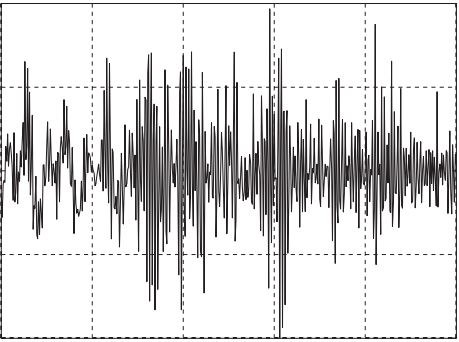
\includegraphics[scale=1]{SignalParole.jpg}
\captionof{figure}{Visualisation d'un signal de parole sur une durée de 1/16 de seconde \cite{Tsa}}
\label{FigParole}
\end{center}
Considérons le signal de parole représenté à la figure \ref{FigParole}. Il est clair, à la vue de ce graphe, que l'on ne peut réduire ces observations à une fonction déterministe du temps. Nous pourrions peut-être trouver une fonction déterministe qui approxime correctement les valeurs observées sur un intervalle de temps $ [0,T] $, mais cette fonction ne serait pas une approximation valable de l'observation à l'extérieur de cet intervalle, et cette propriété perdurerait indépendamment de la durée $ [0,T] $ de l'observation. Le graphe \ref{FigParole} contient un très grand nombre d'irrégularités et ces irrégularités ne semblent pas respecter une évolution prédictible. Les observations ont un caractère aléatoire, dans le sens où nous ne savons pas déterminer, pour un instant donné, quelle sera la valeur précise de la mesure. Par contre, il est envisageable d'indiquer un intervalle de valeurs possibles et éventuellement de préciser comment ces valeurs sont distribuées à partir d'une certaine loi de probabilité.\\
La bonne façon de décrire le comportement du phénomène est donc de spécifier, à chaque instant, une distribution de probabilité, permettant de décrire la vraisemblance de chaque observation. Dans le langage des probabilités, la valeur observée sur le capteur à chaque instant est une variable aléatoire et son évolution au cours du temps, un processus aléatoire. Cet exemple est le prototype d'une large classe de phénomènes qui conduit à adopter, pour les modéliser, la prise en compte de l'indéterminisme \cite{Tsa}.
\paragraph{}
Les signaux aléatoires sont donc en bref des signaux dont la valeur instantanée est imprévisible, ce qui implique qu'ils n'ont pas de représentation analytique. Ces signaux seront étudiés grâce à certains paramètres statistiques qui leur sont associés. C'est en fait ces types de signaux qui sont rencontrés dans notre contexte et nous en reparlerons de manière plus approfondie, mais implicite, dans les parties qui vont suivre.
\subsection{Cas des signaux discrets}
Nous aborderons ici les signaux discrets de manière secondaire. C'est-à-dire, en les prenant comme le résultat de l'\emph{échantillonnage} d'un signal continu, vu que c'est cet aspect qui nous intéressera dans le présent travail.
\subsubsection{Echantillonnage}
Echantillonner\footnote{C'est l'une de manières les plus simples de discrétiser un signal} un signal consiste à prélever, à intervalle de temps régulier le plus souvent, les valeurs prises par le signal. Cela permet ainsi de voir le signal comme une suite de nombres et en permet le traitement par un ordinateur ou tout autre système de traitement des données. C'est en fait le processus de \emph{conversion analogique-numérique}.\\
De manière formelle donc, si on prélève les valeurs du signal avec une période $ T_{e} $, on aura une suite des nombres valant $ \{ s(nT_{e}) \}_{n \in \mathbb{Z}} $ \footnote{De manière tout à fait générale, sans prendre en compte dans un premier temps la causalité (c'est-à-dire le fait selon lequel le temps doit uniquement être pris positif)} qui constitue les échantillons du signal. Par ce fait même, on est amené à songer au problème de reconstitution du signal à partir de ses échantillons. Avant de considérer ce problème, définissons l'impulsion de Dirac qui nous sera très utile pour la suite du travail même si elle n'est pas physiquement réalisable de manière parfaite car elle est idéale.
\paragraph{Impulsion de Dirac\cite{TraitSignMath} :}
Un Dirac $ \delta(t) $ est par définition \emph{une distribution} dont le support (domaine non nul) est réduit au point $ t = 0 $ et d'intégrale valant 1. Formellement, il est défini par:
\begin{eqnarray}
\int_{-\infty}^{+\infty}\delta(t)\,dt = 1
\end{eqnarray}
Ce qui veut dire que cela correspond à un signal de durée nulle et de surface $ 1 $. C'est en fait une limite définie pratiquement par \cite{Unified}:
\begin{eqnarray}
\delta(t) = \lim_{T \to 0}
\begin{cases}
\dfrac{1}{T} & \text{  pour  $ \lvert \dfrac{t}{T} \rvert <\dfrac{1}{2} $}\\
0 & \text{  pour  $ \lvert \dfrac{t}{T} \rvert >\dfrac{1}{2} $} 
\end{cases}
\end{eqnarray}
De cela on peut montrer que:
\begin{eqnarray}
\int_{-\infty}^{+\infty}s(t).\delta(t)\,dt = s(0)
\end{eqnarray}
Comme $ \delta(t-\tau) $ représente une impulsion de Dirac localisée plutôt en $ \tau $, on aura que:
\begin{eqnarray}\label{FonctionVsDirac}
\int_{-\infty}^{+\infty}s(t).\delta(t-\tau)\,dt = s(\tau)
\end{eqnarray}
On remarque que cette manipulation permet de prélever des valeurs de $ s(t) $ en des instants $ \tau $ bien précis. Plus généralement, introduisons un opérateur complet d'échantillonnage nommé \emph{peigne de Dirac} (plusieurs Dirac étendus sur toute la droite des réels et espacés chaque fois de $ \tau $ secondes). Il sera donné par:
\begin{eqnarray}\label{peigneDirac}
c(t) = \sum_{n=-\infty}^{+\infty}\delta(t-n\tau)
\end{eqnarray}
$ c(t) $ permet de réaliser complètement l'échantillonnage d'un signal $ s(t) $ car avec lui on prélève à intervalle de temps régulier $ \tau $ (période d'échantillonnage), la valeur correspondante du signal. En effet, le signal échantillonné est alors donné par \emph{la distribution}:\\
$ s_{e}(t) = \sum_{n=-\infty}^{+\infty}s(nT_{e})\delta(t-nT_{e})
= \sum_{n=-\infty}^{+\infty}s(t)\delta(t-nT_{e})
= s(t)\sum_{n=-\infty}^{+\infty}\delta(t-nT_{e}) $\\
En bref, au vu du développement qui vient d'être fait, on a:
\begin{eqnarray}\label{SignEchantillonDirac}
s_{e}(t) = s(nT_{e}) = s(nT_{e}).c(t) = s(t).c(t)
\end{eqnarray}
Echantillonner un signal revient donc juste à le multiplier par le peigne de Dirac.
\paragraph{Condition d'échantillonnage correct:}
La reconstitution du signal à partir de ses échantillons n'est réalisable que sous certains critères dont le \emph{théorème d'échantillonnage} dit \emph{théorème de Nyquist-Shannon}. Ce théorème donne une condition sur le support du spectre (donné par la transformée de Fourier) du signal $ s(t) $ pour reconstituer $ s(t) $ à partir de ses échantillons $ s(nT_{e}) $. Ce théorème est ainsi énoncé \cite{beal2012theorie}:
\begin{theorem}[Nyquist-Shannon]\label{TheoShannon}
Soit $ s(t) $ un signal dont la transformée de Fourier $ \mathbb{S}(\omega) $\footnote{$ \omega $ représentant la pulsation du signal, avec $ \omega=2.\pi.f $} est à support dans $ [-\frac{\pi}{T_{e}},\frac{\pi}{T_{e}}] $. Alors $ s(t) $ peut être reconstruit en interpolant sur ses échantillons
\begin{eqnarray}
s(t) = \sum_{n=-\infty}^{+\infty}s(nT_{e}).h_{T_{e}}(t-nT_{e})
\end{eqnarray}
Avec
\begin{eqnarray}
h_{T} = sinc(\frac{{\pi}t}{T}) = \frac{\sin\frac{\pi t}{T}}{\frac{\pi t}{T}}
\end{eqnarray}
\end{theorem}
Le théorème nous donne une condition sur  $ \omega $ pour que la reconstitution du signal à partir de ses échantillons soit possible. Cette condition est en effet $ | \omega | \leq \frac{\pi}{T_{e}} $ ce qui veut dire que la fréquence devra vérifier $ f_{max} \leq \dfrac{f_{e}}{2} \Rightarrow f_{e} \geq 2.f_{max} $. En bref, le théorème \ref{TheoShannon} nous dit que \emph{la reconstitution du signal à partir de ses échantillons n'est possible que si la fréquence d'échantillonnage $ f_{e} $ est supérieure ou égale au double de la fréquence maximale du spectre associé au signal}.
\subsubsection{Transformée de Fourier \cite{TraitSignMath}}
Pour un signal discret $ s(nT_{e}) $, la transformée de Fourier est définie par :
\begin{eqnarray}
\mathbb{S}_{d}(f) = \sum_{n = -\infty}^{+\infty}s(nT_{e}).e^{-i.2 \pi f.n}
\end{eqnarray}
C'est au fait la transformée de Fourier de sa représentation sous forme de distribution telle que donnée par \ref{SignEchantillonDirac}.\\
On sait pourtant qu'à un point de vu réel on n'a qu'un nombre fini $ N $ d'échantillons. Pour prendre cela en compte, on définit la transformée de Fourier pour le cas des \emph{signaux finis}. Elle est évidemment donnée par:
\begin{eqnarray}\label{TrFourFinie}
\mathbb{S}_{d}(f) = \sum_{n = 0}^{N-1}s(nT_{e}).e^{-i \frac{2 \pi n}{N} f}
\end{eqnarray}
Cela veut dire que la transformée inverse pour le cas des signaux discrets finis sera donnée par:
\begin{eqnarray}
s(nT_{e}) = \frac{1}{N}\sum_{k = 0}^{N-1}\mathbb{S}_{d}(f).e^{i \frac{2 \pi k}{N} n}
\end{eqnarray}
Cette nouvelle définition( faite en \ref{TrFourFinie}) permet d'introduire en substance un algorithme de calcul \emph{rapide} de la transformée de Fourier. Cet algorithme est largement utilisé par les processeurs spécialisés dans le traitement du signal (les \textbf{DSP}).
\paragraph{Transformée de Fourier Rapide:}On parle souvent d'algorithme FFT.\footnote{Fast Fourier Transform (\textbf{FFT})}\\
C'est une méthode pour calculer la transformée de Fourier discrète d'un signal permettant de réduire le temps de calcul. Pour cela, on calcule la transformée sur une moitié de l'échantillon puis sur l'autre, réduisant ainsi la complexité de l'algorithme de recherche de la transformée. Plus précisément, cet algorithme réduit le nombre d'opérations nécessaires au calcul de la \emph{transformée de Fourier Discrète} de  $ N^{2} $  avec la méthode ordinaire à  $ N\log_{2}{N} $  opérations en utilisant la FFT \cite{Unified}. Comme montré précédemment, c'est utilisé pour le cas de signaux discrets périodiques (signaux discrets finis périodisés comme va le montrer clairement l'explication de l'expression \ref{ConvolutionCirculaire}).  Ici nous n'en donnons qu'une vue sommaire étant donné que dans la suite du travail nous en reparlerons de manière plus claire quoi qu'implicite (voir le point \ref{Butterfly}).\newpage
\section{Filtrage}
\subsection{Introduction}\label{Convol}
Introduisons juste une opération qui nous sera très utile dans la suite.
Filtrer un signal c'est lui faire subir une transformation bien particulière impliquant l'extraction d'une partie qu'on juge utile. En effet, la fonction d'un filtre est de modifier le contenu fréquentiel du signal d'entrée en transmettant intégralement le spectre du signal d'entrée sur certaines gammes de fréquences, et en bloquant le signal d'entrée pour les autres fréquences.  Approximons un filtre par \textit{\emph{un système} linéaire, homogène, invariant et stable}\cite{TraitSignMath}. Au point de vu formel ,le passage d'un signal à travers un filtre implique à ce qu'on lui fasse subir l'action d'un opérateur linéaire, homogène, invariant et stable.\\
De ce fait, considérons un filtre représenté par un opérateur linéaire $ L $. Au vu de ce que nous suggère la définition de l'impulsion de Dirac, se référant plus précisément à l'expression \ref{FonctionVsDirac}, nous voyons que:
\begin{eqnarray}
s(t) = \int_{-\infty}^{+\infty}s(u).\delta(u-t)\,du
\end{eqnarray}
En lui appliquant l'opérateur \emph{linéaire} $ L $, ce qui équivaut à le faire passer à travers un filtre,sans ignorer que $ \delta(t) = \delta(-t) $, on trouve:
\begin{eqnarray}\label{OperateurSurSignal}
L(s(t)) = L\{ \int_{-\infty}^{+\infty}s(u).\delta(t-u)\,du \} = \int_{-\infty}^{+\infty}s(u).L\{\delta(t-u)\}\,du
\end{eqnarray}
Etant donné que $ L $ est aussi homogène en temps, on a que, si $ L\{\delta(t)\} = h(t) $ alors $ L\{\delta(t-u)\} = h(t-u) $. Nous voyons évidemment que $ h(t) $ représente \emph{la réponse du système considéré à une impulsion de Dirac}\footnote{C'est-à-dire le signal observé à la sortie du système en ayant appliqué une impulsion de Dirac en entrée.}. C'est ainsi que \ref{OperateurSurSignal} donne:
\begin{eqnarray}
L(s(t)) = \int_{-\infty}^{+\infty}s(u).h(t-u)\,du
\end{eqnarray}\newpage
C'est la définition du \emph{produit de convolution} du signal par la réponse impulsionnelle du filtre. En bref, faire passer un signal à travers un filtre linéaire et homogène consiste à faire le produit de convolution du signal par la réponse du filtre à une impulsion. Soit dit en passant, le produit de convolution de $ s(t) $ par $ h(t) $ est donné par:
\begin{eqnarray}\label{ConvolutionDef}
s(t)\star h(t) = \int_{-\infty}^{+\infty}s(u).h(t-u)\,du = \int_{-\infty}^{+\infty}s(t-u).h(u)\,du
\end{eqnarray}
La convolution discrète est définie de façon analogue (c'est-à-dire en remplaçant les signaux continus par les correspondants échantillonnés et les intégrales par des sommations discrètes). Toutefois, pour le cas des signaux finis, on définit plutôt \emph{la convolution circulaire} car l'application de la relation précédente comme telle impliquerait la prise en compte des échantillons précédant le début de l'échantillonnage (valeur négative du temps). Pour cela, on considère que l'échantillon observé se répète à l'infini (périodisation des données récoltées). Donc, si $ N $ est le nombre d'échantillons, on devra faire tous les calculs sur $ \mathbb{Z}_{N} $. D'où la définition\cite{TraitSignMath} de la convolution circulaire\footnote{La seule qui soit utilisable en pratique car définie pour les signaux finis.}:\\
En posant $ \dot{n} = n $ $ modulo $  $ N $ car nous travaillons dans $ \mathbb{Z}_{N} $,
\begin{eqnarray}\label{ConvolutionCirculaire}
s(nT_{e}) \circledast h(nT_{e}) = \sum_{p=0}^{N-1}s(\dot{p}T_{e}).h[\dot{\widehat{(n-p)}}.T_{e}]
\end{eqnarray}

La définition du produit de convolution ainsi donnée nous permet de donner un complement fondamental au paragraphe \ref{InteretFourier}. Nous constatons en fait que les exponentielles $ e^{i2 \pi ft} $ sont des \emph{vecteurs propres} des opérateurs de convolution qui sont sans doute des opérateurs linéaire ($ L $ selon notre notation).\\
En effet, appelons $ L(\bullet) $ l'opérateur de convolution défini par $ L(\bullet) = h(t) \star \bullet $. Nous aurons, à la lumière de la définition donnée par l'expression \ref{ConvolutionDef} alliée à la définition de la transformée de Fourier donnée en \ref{TrFourier}:
\begin{eqnarray}
L(e^{i2 \pi ft}) = \int_{-\infty}^{+\infty}h(u).e^{i2 \pi f(t-u)}\,du = (e^{i2 \pi ft}).\mathbb{H}(f)
\end{eqnarray}
Avec $ \mathbb{H}(f) $ la transformée de Fourier de la réponse impulsionnelle $ h(t) $ du filtre $ L $. On le nomme \emph{fonction de transfert du filtre L}. En toute évidence, les exponentielles $ e^{i2 \pi ft} $ sont les vecteurs propres de l'opérateur linéaire $ L $ et les fonctions de transfert associées sont les \emph{valeurs propres} correspondantes.\\
Cela dit, il est tout à fait clair que \emph{c'est plus intéressant d'exprimer tout signal comme somme d'exponentielles complexes pour faciliter les calculs en cas de filtrage, vu que ce dernier est exprimé par un opérateur dont les vecteurs propres sont des exponentielles}. D'où l'intérêt de la série de Fourier et par ricochet, la transformée de Fourier.
\subsection{Prélude au filtrage adaptatif}
Nous ne traiterons pas du filtrage classique ni dans un cadre discret ni dans un cadre continu vu que ce ne sera vraiment pas utile. Nous parlerons néanmoins du \textbf{\emph{filtrage adaptatif}} dont les concepts nous seront d'une grande utilité dans le cadre du présent travail. Pour cela, introduisons d'abord un filtrage particulier qui permettra d'aborder le filtrage adaptatif.
\subsubsection{Filtrage de Wiener\cite{Fmy}}
Ce type de filtrage est conçu pour séparer le signal d'avec le bruit comme tout autre type de filtrage. C'est-à-dire, séparer deux signaux à caractéristiques statistiques différentes.\\
Soient $ s(nT_{e}) $ le signal d'excitation que nous noterons juste $ s(n) $ par commodité(comme pour tous les autres signaux échantillonnés considérés dans ce paragraphe), $ y(n) $ signal qu'on voudrait obtenir à la sortie du système (entaché de bruit normalement), $ e(n) $ le bruit inconnu, $ y_{w}(n) $ le signal modélisé à l'aide des paramètres du filtre, $ \varepsilon (n) $ l'écart entre $ y(n) $ et $ y_{w}(n) $.\\
%\textbf{FIGURE FILTRAGE DE WIENER 000 A LIRE COMP...}\\
Considérant que le signal passe par un système linéaire et homogène, nous aurons à la sortie un signal obtenu par convolution discrète du signal d'entrée avec la réponse impulsionnelle du filtre constituant le système considéré. Il existe donc les coefficients $ w_{k} $ tel que:
\begin{eqnarray}\label{ConvolutionWiener}
y_{w}(n) = \sum_{k=0}^{p-1}w_{k}.s(n-k)
\end{eqnarray}
Ce filtre est à réponse impulsionnelle finie de longueur $ p $ .\\
Notez que, bien que non mentionné, cette convolution est faite avec les mêmes considérations que celles mentionnées pour la \emph{convolution circulaire} donnée en \ref{ConvolutionCirculaire} sauf qu'ici, nous faisons abstraction des \emph{modulos} pour ne pas alourdir l'écriture. Le problème ici consiste à minimiser l'erreur d'estimation approximative $ \varepsilon (n) $ \footnote{On dit \emph{approximative} car la sortie voulue n'est connue qu'à travers un transducteur (qui introduit également un bruit de fond). On minimise plutôt le carré de cette erreur pour des raisons tout à fait pratiques et calculatoires\cite{Esiee}.}.
%\textcolor{red}{Citer 000 A LIRE COMP...}
Nous allons utiliser les notations matricielles pour être général (en ce qui concerne le nombre de coefficients du filtre en particulier). La relation \ref{ConvolutionWiener} devient:
\begin{eqnarray}
y_{w}(n) = \sum_{k=0}^{p-1}w_{k}.s(n-k) = W^{T}.S(n) =S(n)^{T}.W 
\end{eqnarray}
Avec $ W = $
\(
\begin{pmatrix}
w_{0} & w_{1} & \cdots & w_{p-1}
\end{pmatrix}
\)$ ^{T} $
;\\
$ S(n) = $
\(
\begin{pmatrix}
s(n) & s(n-1) & \cdots & s(n-p+1)
\end{pmatrix}
\)$ ^{T} $\\
et l'exposant $ T $ sur les vecteurs indique qu'on a fait la transposition.\\
De là on tire:
\begin{eqnarray}
\varepsilon^{2}(n) = [y(n)-S(n)^{T}.W]^{2} = y(n)^{2}-2y(n)S(n)^{T}W + W^{T}S(n)S(n)^{T}W
\end{eqnarray}
Appelons $ \Gamma(W) $ la valeur moyenne des erreurs commises (avec $ \mu $ l'opérateur indiquant qu'on fait une moyenne). C'est elle qu'il nous faudra chercher à minimiser pour espérer trouver un filtre optimal. Au vu du développement précédent nous aurons:
\begin{eqnarray}\label{FonctionCoût}
\Gamma (W) = \mu \{y(n)^{2}\} - \mu \{2y(n)S(n)^{T}W\} + \mu \{W^{T}S(n)S(n)^{T}W\}
\end{eqnarray}
Dérivons $ \Gamma(W) $ par rapport à $ W $ (ce qui correspond plus précisément à la recherche du gradient), ça donne:
\begin{eqnarray}\label{BrouillonHopf}
\frac{d[\Gamma (W)]}{dW} = - 2\mu \{y(n)S(n)^{T}\} + 2\mu \{S(n)S(n)^{T}\}.W
\end{eqnarray}
Notons que   $ \mu \{y(n)S(n)^{T}\} = $  
\(
\begin{pmatrix}
\dfrac{1}{N} \sum_{n=0}^{N-1}y(n).s(n) \\
\dfrac{1}{N} \sum_{n=0}^{N-1}y(n).s(n-1)\\
\vdots \\
\dfrac{1}{N} \sum_{n=0}^{N-1}y(n).s(n-p+1)
\end{pmatrix}
\)\\
avec $ N $ le nombre d'échantillons (Idem pour les autres moyennes, sachant que la moyenne d'une matrice consiste à faire l'opération pour tous ses termes).\\
Rappelons que:
\begin{itemize}
\item[•] $ \mu \{y(n)S(n)^{T}\} $ est un vecteur de dimension $ p $ (vu que $ y(n) $ est un simple scalaire à chaque fois),on le nomme \emph{vecteur d'intercorrélation} et nous le noterons $ R_{sy} $.
\item[•] $ \mu \{S(n)S(n)^{T}\} $ est une matrice $ p\times p $ nommée \emph{matrice d'autocorrélation} et nous la noterons $ R_{ss} $.
\end{itemize}
Par conséquent, comme le minimum se retrouve en annulant le gradient, de l'expression \ref{BrouillonHopf} on tire l'équation donnant les coefficients $ w_{k} $ lorsque la dérivée est nulle, donc le filtre optimal $ W_{opt} $. On a:
\begin{eqnarray}\label{EquationWienerHopf}
R_{ss}.W = R_{sy} \Rightarrow W_{opt} = R_{ss}^{-1}.R_{sy}
\end{eqnarray}
C'est l'\emph{équation normale} dite de \emph{Wiener-Hopf}.

On remarque évidemment qu'implémenter ce système aura un certain nombre de lacunes dont par exemple le temps de calcul des matrices ainsi que l'espace mémoire nécessaire surtout pour l'inversion de la matrice $ R_{ss} $. Le problème le plus pertinent est que \emph{si les signaux ne sont pas stationnaires, ce qui est pourtant plus fréquemment le cas pour les signaux réels, $ R_{ss} $ et $ R_{sy} $ évoluent au cours du temps. Cela veut dire qu'il faudra chaque fois résoudre à nouveau l'équation de Wiener-Hopf}.\\
Ce qui vient d'être montré justifie qu'il est impérieux de trouver un moyen efficace pour pouvoir résoudre récursivement et plus rapidement l'équation de Wiener-Hopf. Le filtrage adaptatif apporte une solution efficace à ce problème.
\section{Traitement du signal audio}
Le traitement du signal audio est un domaine très vaste qu'on ne peut espérer aborder de manière exhaustive dans ce document. Premièrement, cela serait une perte d'énergie et deuxièmement c'est une entreprise utopique. Le son peut en fait subir divers traitements dont le filtrage. Nous nous intéressons juste au filtrage ayant pour finalité l'annulation d'un écho présent dans le fichier sonore.\\
L'annulation d'écho est ardue si on l'étudie de manière détaillée, c'est-à-dire en voulant considérer tous les paramètres qui entrent en jeu. En effet, pour annuler l'écho, il faut connaître précisément le milieu de propagation du son qu'on veut débarrasser de la perturbation en question. Le problème est qu'en premier, une telle étude serait irréalisable car cela prendrait en compte un très grand nombre de paramètres. En second lieu, les paramètres varieraient continuellement dans le temps (considérer pour cela le fait que, dans une enceinte, le changement de positon de l'un des éléments a une influence significative sur le comportement de ladite enceinte par rapport au signal à considérer; par exemple, le déplacement du microphone modifie directement la réponse de l'enceinte au signal et change par là même les calculs à faire pour annuler au mieux l'écho,...) et cela rendrait juste l'entreprise irréaliste.

Une solution plus pratique serait d'aborder le problème de manière globale, en considérant plutôt l'enceinte comme un système dont il suffirait juste d'étudier le comportement, grâce à un modèle équivalant, qui faciliterait le traitement par des algorithmes de calcul et diminuerait ainsi le nombre de paramètres pris en compte. Cela rendrait l'étude systématique réalisable en pratique. Au vu de ce dont nous avons parlé dans les sections précédentes, la solution est d'étudier la fonction de transfert associée à l'enceinte considérée et de recourir au filtrage adaptatif pour une prise en compte efficace de l'évolution temporelle du système. La stratégie d'annulation d'écho acoustique repose sur une estimation du canal acoustique de l'écho en identifiant la réponse impulsionnelle du bouclage acoustique qui est retranchée finalement du signal.\\
Le filtrage étant adaptatif, les coefficient du filtre sont adaptés en fonction de l'erreur commise à chaque itération. La réponse impulsionnelle du filtre varie au cours du temps et dépend du signal en entrée, de la séquence d'apprentissage et de l'algorithme d'optimisation choisi\cite{ThAlaedine}.
\section{Conclusion partielle}
Dans ce premier chapitre, nous avons premièrement justifié le bien fondé de l'application de l'analyse de Fourier au traitement du signal tout en pointant les résultats intéressants de cette dernière discipline.\\
Deuxièmement, nous avons montré de manière implicite à quel point le traitement numérique du signal est fécond et intéressant. En effet, il facilite les manipulations à effectuer sur les signaux, en facilite l'étude théorique et surtout, est plus adaptable aux divers systèmes de traitement des données existant, tout en étant moins sensible aux caprices de la nature (insensibilité du signal,  dès qu'il est numérisé, aux perturbations de l'appareillage).\\
Nous y avons également traité du filtrage adaptatif. Pour cela, le concept a été illustré par le filtre de Wiener (filtre en général non utilisable pour le son car restreint aux signaux stationnaires), très crucial pour le développement du filtrage adaptatif proprement-dit qui est abordé dans le chapitre qui suit.
\chapter{ÉTUDE THÉORIQUE DU FILTRAGE DU SON}
\section{Introduction partielle}
Le traitement du signal sonore doit être minutieusement réalisé car les effets d'un mauvais traitement sont facilement perceptibles. Un traitement particulier, le filtrage, avec comme objectif d'annuler l'écho éventuel du signal sonore, fait l'objet de ce chapitre. Nous avons principalement opté pour un traitement numérique du signal à cause des avantages que cela procure (allant de la facilité de traitement à la facilité de réplique des manipulations effectuées en passant par la grande disponibilité des concepts élaborés du domaine).\\
C'est ainsi que nous présentons, en premier lieu, divers algorithmes de filtrage conçus principalement avec comme objectif d'aboutir à une possibilité d'annuler l'écho d'un signal sonore.\\
En second lieu, nous abordons un type de transformation numérique particulier, la transformée en nombres de Fermat, qui constitue un substitut valable à la transformation de Fourier discrète dans des situations où il est impérieux de réduire la complexité de calcul des algorithmes élaborés.\\
En troisième et dernier lieu, nous y présentons un paradigme très essentiel pour une réduction encore plus grande de la complexité des algorithmes élaborés pour le traitement des signaux. Il s'agit du traitement par bloc des séquences numériques.\\
\section{Quelques algorithmes de filtrage adaptatif}
Le filtrage adaptatif a été introduit à la fin du premier chapitre. En gros, ça consiste à réaliser le filtrage avec un filtre numérique qui change et s'adapte à l'enceinte selon un critère bien défini (un critère de minimisation du carré de l'erreur d'estimation par exemple). Pour cela nous avons parlé du filtre de Wiener qui, bien que n'étant utilisable qu'en cas des signaux stationnaires, nous permet d'aborder de manière claire et succincte le filtrage adaptatif.\\
Ces algorithmes ont donc pour raison d'être l'approximation du filtre optimal de Wiener en cas des signaux non stationnaires. Il s'agit du \emph{filtrage adaptatif proprement-dit}.
\subsection{Algorithme du gradient déterministe}
L'équation de Wiener-Hopf vue à la fin du précédent chapitre permet de retrouver le filtre optimal en résolvant un système de $ p $ équations à $ p $ inconnues. Cet algorithme permet de résoudre le système de manière itérative. Cela est fait en deux étapes:
\begin{itemize}
\item Choix du vecteur $ W_{0} $ ($ W $ initial).
\item Obtention, à partir de $ W_{k} $ , de $ W_{k+1} $ par incrémentation de $ W_{k} $ dans la direction opposée au gradient de la fonction moyenne des erreurs $ \Gamma(W) $ introduite en \ref{FonctionCoût}.
\end{itemize}
Ainsi on aura\cite{Esiee}:
\begin{eqnarray}
W_{k+1} = W_{k} - \frac{1}{2}\lambda\nabla [\Gamma(W)]
\end{eqnarray}
Et pourtant on sait que, selon les notations adoptées, et suite à l'égalité \ref{BrouillonHopf} on a:
\begin{eqnarray}
\overrightarrow{grad}\Gamma(W) \equiv \nabla [\Gamma(W)] = \frac{d[\Gamma(W)]}{dW} = -2R_{sy}+2R_{ss}W_{k}
\end{eqnarray}
Par conséquent, l'\emph{algorithme du gradient déterministe} est donné par\cite{ThAlaedine}:
\begin{eqnarray}\label{AlgoGradDéterministe}
W_{k+1} = W_{k} + \lambda( R_{sy} - R_{ss}.W_{k})
\end{eqnarray}
La stabilité de cet algorithme est contrôlée par le \emph{pas d'adaptation} $ \lambda $, elle dépend également de la matrice d'autocorrélation du vecteur d'entrée\cite{ThAlaedine}.\\
En effet, si on nomme $ E_{k} $ l'écart entre $ W_{k} $ et $ W_{opt} $ après $ k $ itérations, on aura:
\begin{eqnarray}
E_{k} = W_{k} - W_{opt}
\end{eqnarray}
or selon l'équation de Wiener-Hopf,
\begin{eqnarray}
R_{ss}W_{opt} = R_{sy}
\end{eqnarray}
Et selon l'algorithme du gradient déterministe on aura:
\begin{eqnarray}
W_{k+1} &=& W_{k} + \lambda .( R_{ss}.W_{opt} - R_{ss}.W_{k})\\
		&=& W_{k} + \lambda R_{ss}.( W_{opt} - W_{k})\\
		&=& W_{k} - \lambda R_{ss}.E_{k}
\end{eqnarray}
De ce qui précède on tire que
\begin{eqnarray}
E_{k+1} = W_{k+1} - W_{opt} = E_{k} - \lambda R_{ss}.E_{k}
\end{eqnarray}
Ce qui montre de manière évidente de quelle façon la convergence de l'algorithme dépend du pas d'adaptation et de la matrice d'autocorrélation du vecteur d'entrée.\\
\emph{La convergence de l'algorithme} est assurée par la contrainte\cite{Esiee}:
\begin{eqnarray}
0 \lneq \lambda \lneq \frac{2}{\lambda_{pro_{max}}}
\end{eqnarray}
Avec $ \lambda_{pro} $ représentant une quelconque valeur propre de la matrice d'autocorrélation du signal d'entrée et $ \lambda_{pro_{max}} $ la plus grande valeur propre de cette matrice.\\
Notons que pour des faibles valeurs de $ \lambda $ (pas d'adaptation), le temps de convergence lui est inversement proportionnel. Le choix de $ \lambda $ est trop délicat et sa fixité ne garantit pas une vitesse de convergence optimale de l'algorithme. Par conséquent, il est nécessaire d'y trouver une solution.
\subsection{Algorithme du gradient stochastique(LMS) \cite{ThAlaedine}}
Cet algorithme dit des moindres carrés ou LMS (Least Mean Square) consiste à minimiser l'erreur quadratique moyenne. C'est-à-dire en considérant son gradient au lieu de celui de la moyenne des carrés des erreurs (que nous avons nommé $ \Gamma(W) $). Cela résout approximativement le problème évoqué au paragraphe précédent pour l'algorithme du gradient déterministe, problème de faible vitesse de convergence pour des très faibles valeurs du pas d'adaptation. Au fait, c'est plus adapté en pratique car on a très rarement $ \nabla [\Gamma(W)] $.\\ Ainsi, comme $ \nabla [\varepsilon^{2}(n)] = \nabla[\varepsilon_{k}^{2}] = 2\varepsilon_{k}.\dfrac{\partial \varepsilon_{k}}{\partial W} = -2.\varepsilon_{k}.S_{k} $\footnote{$ S_{k} $ représente le vecteur $ S(n) $ à la $ k^{ieme} $ itération et $ \varepsilon_{k} $ l'erreur(c'est un scalaire) $ \varepsilon(n) $ après le même nombre d'itérations.}, on aura l'algorithme LMS donné par:
\begin{eqnarray}\label{AlgoLMS}
W_{k+1} = W_{k} - \frac{1}{2}\lambda\nabla [\varepsilon^{2}(n)] = W_{k} + \lambda S_{k}\varepsilon_{k}
\end{eqnarray}
L'adaptation qui assure la convergence en moyenne quadratique la plus rapide est donnée par\footnote{Avec l'hypothèse d'un \emph{bruit blanc} en entrée}:
\begin{eqnarray}
\lambda_{opt} = \frac{2}{p.\sigma^{2}(s)}
\end{eqnarray}
Avec $ \sigma^{2}(s) $ la \emph{variance du signal d'entrée}.\\
On remarque que la convergence de l'algorithme LMS dépend de la statistique du signal d'entrée. Pour les signaux non stationnaires, il est difficile de suivre les variations du signal d'entrée avec l'adaptation du filtre par l'algorithme LMS et cela donne une convergence lente. D'où l'algorithme des moindres carrés récursif.
\subsection{Algorithme des Moindres Carrés Récursif \cite{ThAlaedine, Esiee}}
Cet algorithme, le \emph{Recursive Least Squares \textbf{RLS}}, permet de suivre les signaux non stationnaires tout en ayant une vitesse de convergence convenable. Ici, au lieu de minimiser un critère statistique établi sur l'erreur commise en estimant un signal, on minimise, à chaque itération la somme des carrés des erreurs commises depuis l'instant initial. Dans ce cas, $ \Gamma(W) $ serait donné par\\ $ \Gamma(W) = \dfrac{1}{k}\sum_{n = 0}^{k}\varepsilon^{2}(n) $ mais vu que cela n'affecte pas le critère de minimisation, on prendra plutôt:
\begin{eqnarray}
\Gamma(W) = \sum_{n = 0}^{k}\varepsilon^{2}(n)
\end{eqnarray}
La réponse $ W $ du filtre adaptatif \emph{est donc fonction des échantillons disponibles et non d'une moyenne statistique générale}. Cela est très capital et constitue le noyau de cet algorithme. Par analogie avec le filtre de Wiener on aura les relations\footnote{C'est logique car les développements sont \emph{formellement} identiques}:
\begin{eqnarray}
R_{ss_{k}}W_{k} = R_{sy_{k}}
\end{eqnarray}
Avec $ R_{ss_{k}} = \sum_{n=0}^{k}S_{n}.S_{n}^{T} $ et $ R_{sy_{k}} = \sum_{n=0}^{k}S_{n}.y(n) $.\\
La réponse impulsionnelle du filtre sera donc modifiée à chaque itération. Pour limiter le nombre des calculs, l'équation à utiliser, et qui constitue l'algorithme RLS, est la suivante:
\begin{eqnarray}\label{AlgoRLS}
W_{k+1} = W_{k} + R^{-1}_{ss_{k}}S_{k}\varepsilon_{k}
\end{eqnarray}
Et dans cette formule, le calcul de $ R^{-1}_{ss_{k}} $ se fait par:
\begin{eqnarray}
R^{-1}_{ss_{k}} = \frac{1}{\delta}[R^{-1}_{ss_{k-1}} - \frac{R^{-1}_{ss_{k-1}}.S_{k}^{T}.R^{-1}_{ss_{k-1}}}{\delta + S_{k}^{T}.R^{-1}_{ss_{k-1}}.S_{k}}]
\end{eqnarray}
Avec $ R_{ss_{0}} = \dfrac{1}{\delta}.I_{p}$ avec \emph{$ I_{p} $ matrice unité de dimension $ p\times p $ },  $ \delta \in\, \rbrack 0,1 \lbrack $ et $ W_{0} \equiv $ \emph{vecteur nul de dimension $ p $ }.\\
Cet algorithme converge plus vite que le LMS mais est plus difficile à mettre au point. Un palliatif à cette difficulté de mise en application est l'algorithme dit NLMS.
\subsection{Algorithme LMS Normalisé (NLMS) \cite{ThAlaedine, Fmy}}
Le \emph{Normalized Least Mean Square} dit NLMS pallie à la complexité du RLS et, de manière directe et plus globale, à l'inadaptation du coefficient d'adaptation de l'algorithme LMS (Problème soulevé à la fin du paragraphe sur l'algorithme LMS). Cet algorithme consiste à normaliser le coefficient d'adaptation $ \lambda $ du LMS en prenant en compte l'énergie du signal d'entrée, ce qui réduit au minimum l'effet de l'influence de la variation de la puissance du signal. Cela rend la vitesse de convergence plus ou moins uniforme en passant d'une itération à l'autre. Donc on aura la même formule d'itération que celle donnée pour l'algorithme LMS par l'équation \ref{AlgoLMS}, à la différence près que le coefficient d'adaptation est ainsi normalisé:
\begin{eqnarray}
\lambda_{k} = \frac{\lambda}{S_{k}^{T}.S_{k} + \beta}
\end{eqnarray}
Par conséquent, l'algorithme NLMS est donné par l'équation:
\begin{eqnarray}\label{AlgoNLMS}
W_{k+1} = W_{k} + \frac{\lambda}{S_{k}^{T}.S_{k} + \beta}.S_{k}\varepsilon_{k}
\end{eqnarray}
$ \beta $ est un facteur permettant de suivre rapidement les variations de l'énergie dans le signal d'entrée.\\
La convergence de cet algorithme est garantie si $ \lambda_{k} \in\, \rbrack 0,\dfrac{2}{\lambda_{pro_{max}}} \lbrack $. L'intérêt de cet algorithme par rapport au LMS est qu'il est indépendant à la variance du signal d'entrée. Il faudra toutefois noter qu'ici aussi il y a dépendance de la convergence de l'algorithme à la statistique du signal d'entrée car la distribution des valeurs propres de la matrice d'autocorrélation du signal n'est pas modifiée. Pour les signaux stationnaires (le \emph{bruit blanc}  par exemple) ou non-stationnaires (signal de \emph{parole} par exemple), le NLMS apporte une amélioration significative du taux de convergence suite à la normalisation. En ce qui concerne la mise en œuvre, cet algorithme est plus complexe que le LMS mais en pratique il fait partie des plus simples et plus efficaces algorithmes d'adaptation.
\subsection{Algorithme Proportionné Normalisé (PNLMS)\cite{ThAlaedine}} \label{MatrGk}
Cet algorithme, le PNLMS, spécialement adapté à l'annulation d'écho, fait l'adaptation avec un taux de convergence variable. Il a plus d'opérations que le NLMS mais converge plus vite; il découle du NLMS en remplaçant le $ \lambda_{k} $ par:
\begin{eqnarray}
\lambda_{k} = \frac{\lambda G_{k}}{S_{k}^{T}.G_{k}.S_{k} + \beta}
\end{eqnarray}\newpage
Avec $ G_{k} = diag[g_{k}(0),\cdots ,g_{k}(p-1)] $ qui est une matrice diagonale de type $ p\times p $.\\
Et chaque fois, $ g_{k}(n) = \dfrac{\gamma_{k}(n)}{\dfrac{1}{p}\sum_{m=0}^{p-1}\gamma_{k}(m)} $ où $ \gamma_{k}(n) = \max\{\rho \nu_{k}, |w_{k}(n)|\} $ , $ n \in \, \{0,\cdots ,p-1\} $ et $ \nu_{k} = \max\{\delta,|w_{k}(0)|, \cdots ,|w_{k}(p-1)|\} $. Les termes $ \rho $ et $ \delta $ valent respectivement $ \dfrac{5}{p} $ et $ 10^{-2} $ . Donc l'algorithme PNLMS est donné par:
\begin{eqnarray}\label{AlgoPNLMS}
W_{k+1} = W_{k} + \frac{\lambda G_{k}}{S_{k}^{T}.G_{k}.S_{k} + \beta} \cdot S_{k}\varepsilon_{k}
\end{eqnarray}
Néanmoins, sous certaines conditions dont la \emph{dispersivité de la réponse du filtre adaptatif}, le PNLMS devient moins rapide que le NLMS. La solution à ce problème est la combinaison de ces deux algorithmes. D'où l'algorithme nommé \textbf{PNLMS++}.
\subsection{Algorithme PNLMS++ \cite{ThAlaedine}}
Cet algorithme est moins sensible aux variations de la réponses impulsionnelle du filtre. Il consiste à combiner les deux précédent comme suit:
\begin{itemize}
\item[•] Pour les itérations de numéro impair ($ k $ impair), utilisation du PNLMS.
\item[•] Pour les itérations paires, on utilise le NLMS. 
\end{itemize}
Puis en fin de compte on mélange les résultats pour retrouver le filtre optimal.\\
 \\
L'algorithme ainsi défini est celui que nous utiliserons. Toutefois, il subira un certain nombre de modifications pour pouvoir devenir plus manipulable et plus optimal. Ces manipulations seront effectuées en faisant en sorte que les calculs puissent s'effectuer sur un processeur de traitement numérique des signaux sans oublier de prendre en compte le coût, la rapidité et la minimisation d'erreurs. Ainsi, nous devons chercher comment réaliser les opérations voulues en utilisant un \emph{processeur à virgule fixe}, pour ne pas avoir à gérer les erreurs d'arrondissement introduites par une manipulation maladroite du \emph{processeur à virgule flottante}, tout en réduisant le coût d'achat du matériel (le premier processeur étant moins cher que le second). Pour cela, une transformation tout à fait particulière nous sera utile; il faudra juste qu'elle ait les mêmes propriétés qu'une transformation de Fourier (surtout en ce qui concerne la convolution) et qu'elle rende les calculs (le traitement) plus optimisé. On le réalise grâce à la transformation qui fait l'objet de la section qui suit.
\section{Transformée en nombres entiers (NNT) \cite{ThAlaedine}}
La transformée en nombres entiers a la même forme que la transformée de Fourier discrète mais la supplante en ce sens que la partie imaginaire n'existe plus dans cette nouvelle transformation. La racine primitive considérée dans cette dernière (l'exponentiel complexe) étant remplacée par la racine $ M^{ieme} $ de l'unité dans le corps de Galois\cite{Galois}\footnote{Chaque fois le corps de Galois d'ordre $ q $ sera noté $ GF(q) $ selon la  notation anglaise standard.} considéré.\\
Soit $ \alpha $ cette racine. Nous avons donc que
\begin{eqnarray}
\langle\alpha^{M} = 1\rangle_{q}
\end{eqnarray}
Avec $ \langle \cdot \rangle_{q} $ signifiant que le calcul est fait \emph{modulo q}, c'est-à-dire dans un corps de Galois d'ordre $ q $. La formule précédente est celle qui sera chaque fois utilisée pour retrouver la racine primitive $ \alpha $ dès que $ M $ et $ q $ sont choisis. La transformée en nombres entiers de chaque terme $ x_{n} $ d'une séquence de longueur $ M $ est alors donnée par:
\begin{eqnarray}\label{TransNombEntiers}
X_{k} = \langle\sum_{n=0}^{M-1}x_{n}\alpha^{nk}\rangle_{q}
\end{eqnarray}
Si la longueur de la transformée $ M $ et l'ordre $ q $ du corps fini (sachant que tout corps fini est corps de Galois)\cite{GaloisD} $ GF(q) $ sont premiers entre eux, il existe alors $ ( M^{-1} ) $ \footnote{Des algorithmes de calcul rapide de l'inverse d'un nombre dans un corps fini existent et seront présentés dès que nécessaire.} tel que $ \langle M.M^{-1} \equiv 1\rangle_{q} $ (ceci signifie que $ M.M^{-1} $ est congru à $ 1 $ modulo $ q $) et là l'inverse de la transformée existe si $ M\vert(q-1) $ (ça veut dire que $ M $ divise $ q-1 $), elle est donnée par:
\begin{eqnarray}\label{TransInvNombEntiers}
x_{n} = \langle M^{-1}\sum_{k=0}^{M-1}X_{k}\alpha^{-nk}\rangle_{q}
\end{eqnarray}
La transformée en nombres entiers n'existe pas toujours; les conditions de son existence sont les suivantes:\newpage
\begin{itemize}
\item[•] On doit avoir que $ pgcd(\alpha,q) = pgcd(M,q) = 1 $ ce qui implique que $ \langle\alpha^{M} = 1\rangle_{q} $ (existence de la racine primitive $ \alpha $).
\item[•] Si $ q $ est premier, il faut nécessairement que $ M\vert(q-1) $.\\ Sinon $ q=\prod_{i=0}^{k}p_{i}^{m_{i}} $ et $ M\vert pgcd(p_{i}-1,p_{j}-1)$  $ \forall(i,j)\in\{1,2,...\}^{2}$. Avec $ i \neq j $ et $ q=\prod_{i=0}^{k}p_{i}^{m_{i}} $ représentant exactement la décomposition de $ q $ en facteurs premiers.
\item[•] Il faut que $ pgcd((\alpha^{i}-1),q) = 1 $ si $ i $ est un diviseur de $ M $, $ \forall i\in\{1,2,...,M-1\} $
\end{itemize}
\subsection{Choix des paramètres de la transformation et Transformée en nombres de Fermat (FNT)}\label{NbrFermat}
De même que pour la transformée de Fourier discrète, la transformée en nombres entiers demanderait un ordre de $ M^{2} $ multiplications et $ M(M-1) $ additions. L'opération la plus complexe ici est évidemment la multiplication par des puissances de la racine unité $ \alpha $. De cela découle qu'il est impérieux de faire un choix judicieux de cette racine pour réduire la charge de calcul des processeurs à utiliser (il est ainsi plus malin de choisir $ \alpha $ puissance de 2 pour remplacer toutes les multiplications par des décalages de bit). Le choix de l'ordre $ q $ du corps de Galois dans lequel on choisit de travailler est aussi important pour une programmation plus optimale. Il est plus avantageux de prendre un ordre $ q $ égal à \emph{un nombre de Fermat}. C'est-à-dire un nombre de la forme $ 2^{b} + 1 $ avec $ b $ une puissance de 2 car cela rend l'algorithme très optimal. On parle de la \textbf{\emph{transformation en nombres de Fermat}}.
Il s'agit d'une transformée en nombres entiers dans un corps d'ordre égal à un nombre de Fermat (il faut noter en passant que, seuls les 5 premiers nombres de Fermat sont premiers). Ainsi on a que $ q = 2^{2^{t}} + 1 $ avec $ t\in\mathbb{N} $. Cette transformée est celle que nous utiliserons vu qu'elle rend nos algorithmes plus optimisés.
\subsection{Transformation en nombres de Fermat et arithmétique binaire}\label{MetALPHA}
Nous devons analyser la transformation sous cet angle (sous l'angle de l'arithmétique binaire) car cela permet de rester dans notre contexte vu que nos calculs seront exécutés par un processeur numérique fonctionnant sous le même principe.\\
Une FNT (Fermat Number Transform) de longueur quelconque $ M = 2^{t+1} $ a juste $ \frac{M}{2}\log_{2}M $ multiplications et $ M\log_{2}M $ additions. Nous voyons à quel point il est intéressant de travailler dans un corps de Galois ayant un ordre $ q $ égal à un nombre de Fermat $ F_{t} $. Le terme générateur $ \alpha $ étant aussi essentiel à la réduction de la complexité de calcul, le choix d'un $ \alpha $ différent d'une racine primitive (contrairement aux indications du début) mais égal à une puissance de $ 2 $ est intéressant en arithmétique binaire pour réduire la charge de calcul en cas de multiplication. Les longueurs possibles sont alors données par $ M = 2^{t+1-i} $ et $ \langle\alpha = 2^{2^{i}}\rangle_{F_{t}} $ avec évidemment $ (i,t)\in\mathbb{N}^{2} $ tel que $ 0\leqslant i<t $.La longueur de séquence étant égale à une puissance de 2, $ \langle M^{-1} = -2^{2^{t}-1-(t-i)}\rangle_{F_{t}} $ car en effet,
\begin{eqnarray}
\begin{aligned}
\langle F_{t}-1 = 2^{2^{t}} & \equiv  -1\rangle_{F_{t}}\\
\langle 2^{2^{t}}\cdot 2^{-(t-i+1)}  \equiv & -2^{-(t-i+1)}\rangle_{F_{t}}\\
\langle M^{-1} = 2^{-(t+1-i)} & \equiv  -2^{2^{t}-1-(t-i)}\rangle_{F_{t}}
\end{aligned}
\end{eqnarray}
D'où les formules de transformation seront données, à la lumière des relations \ref{TransNombEntiers} et \ref{TransInvNombEntiers}, par:
\begin{eqnarray}
\begin{aligned}
X_{k} &= \langle\sum_{n=0}^{2^{t+1-i}-1}x_{n}\cdot 2^{\langle 2^{i}nk\rangle_{M}}\rangle_{F_{t}}\\
x_{n} &= \langle -2^{2^{t}-1-(t-i)}\sum_{k=0}^{2^{t+1-i}-1}X_{k}\cdot 2^{\langle -2^{i}nk\rangle_{M}}\rangle_{F_{t}}
\end{aligned}
\end{eqnarray}
On peut doubler la longueur des séquences tout en conservant un $ \alpha $ puissance de $ 2 $. Pour cela il suffit de poser que $ i = -1 $. Ainsi la racine $ \alpha $ est solution de la relation de congruence $ \langle\alpha^{2} = 2\rangle_{F_{t}} $. Donc,
\begin{align*}
\alpha^{2} &= \langle 2 = (-1)\cdot 2\cdot (-1) = -2\cdot (-1)\rangle_{F_{t}}\\
&= \langle -2\cdot 2^{2^{t}} = 2^{2^{t-1}}(1-1-2\cdot 2^{2^{t-1}})\rangle_{F_{t}}\\
&= \langle(2^{2^{t-2}})^{2}((2^{2^{t-1}})^{2}-2\cdot 2^{2^{t-1}} + 1^{2})\rangle_{F_{t}}\\
&= \langle(2^{2^{t-2}}(2^{2^{t-1}}-1))^{2}\rangle_{F_{t}}
\end{align*}
Par conséquent, $ \alpha\equiv\sqrt{2}$ a un sens et existe dans le corps de Galois $ GF(q)\equiv GF(F_{t}) $ si et seulement si $ t\geq 2 $ car du développement précédent on tire clairement que:
\begin{eqnarray}
\langle\alpha\equiv\sqrt{2} = {2^{2^{t-2}}} \cdot (2^{2^{t-1}}-1)\rangle_{F_{t}}
\end{eqnarray}
 \\
Donc, $ (\sqrt{2}^{n}) = \left\{\begin{array}{ll}
\langle 2^{\frac{n}{2}}\rangle_{F_{t}} & \mbox{ pour $ n $ pair}\\
\langle 2^{\frac{n-1}{2}}\cdot 2^{2^{t-2}}(2^{2^{t-1}}-1)\rangle_{F_{t}} & \mbox{ sinon }
\end{array}\right. $.\\
 \\
Comme \emph{cette transformation admet que la transformée du produit de convolution de deux séquences est égale au produit simple(terme à terme) des transformées des séquences convoluées}, elle requiert $ M\log_{2}M $ opérations simples (décalage de bit, additions) et \emph{aucune multiplication}. Cela est génial vu que comparativement, la transformée de Fourier discrète requiert, hormis les opérations simples, un nombre de multiplications complexes de l'ordre de $ \frac{M}{2}\log_{2}\frac{M}{2} $.
\subsection{Version rapide de la FNT}\label{Butterfly}
De même qu'il existe une version rapide de la transformée de Fourier (la FFT comme dit au premier chapitre), il en existe aussi une pour la transformée en nombres de Fermat. Le principe est le même et \emph{c'est la même chose du point de vu formel}. Il consiste à diviser la séquence en 2 séquences plus petites, ce qui réduit la complexité des calculs. L'implantation de cet algorithme sur un processeur de calcul porte le nom d'\emph{implantation Butterfly}.\\
Une transformée en nombres de Fermat de dimension $ M = 2^{n} $ avec $ 0 \leq n\leq b = 2^{t} $ peut être calculée en utilisant le principe de l'algorithme FFT de la manière suivante:
\begin{eqnarray}
\begin{aligned}
\langle X_{k} = \sum_{n=0}^{M-1}x_{n}\alpha^{nk} = \sum_{n=0}^{\frac{M}{2}-1}x_{2n}\alpha^{2nk} + \sum_{n=0}^{\frac{M}{2}-1}x_{2n+1}\alpha^{(2n+1)k}\rangle_{F_{t}}\\
\langle X_{k} = \sum_{n=0}^{\frac{M}{2}-1}x_{2n}\alpha^{2nk} + \alpha^{k}\sum_{n=0}^{\frac{M}{2}-1}x_{2n+1}\alpha^{2nk} = G_{k}+\alpha^{k}H_{k}\rangle_{F_{t}}
\end{aligned}
\end{eqnarray}
Avec évidemment $ G_{k} $ et $ H_{k} $ des vecteurs représentant respectivement les transformées en nombres de Fermat des séquences $ \{x_{2n}\}_{n=0}^{\frac{M}{2}-1} $ et $ \{x_{2n+1}\}_{n=0}^{\frac{M}{2}-1} $ de longueur $ \frac{M}{2} $.\\
Comme $ \langle\alpha^{M} = 1\rangle_{F_{t}} \Rightarrow \langle\alpha^{k+\frac{M}{2}} = -\alpha^{k}\rangle_{F_{t}} $ car $ \langle\alpha^{M} = 1 = (-1)^{2} = (\alpha^{\frac{M}{2}})^{2}\rangle_{F_{t}} $.\\
 \\
En fin de compte,$ \left\{\begin{array}{lcl}
X_{k} &=& G_{k} + \alpha^{k}H_{k} \\
X_{k+\frac{M}{2}} &=& G_{k} - \alpha^{k}H_{k}
\end{array}\right. $   $ k\in [0,\frac{M}{2}-1]\subset\mathbb{N} $.\\
 \\
Ce découpage de la séquence en 2 parties égales peut être repété pour décomposer la transformée de longueur $ M = 2^{b} $ en $ \{4,8,\cdots ,\dfrac{M}{2} $ parties. Toute FNT peut ainsi être calculée grâce à $ \log_{2}(2^{b}) = b $ décompositions. Comme $ \frac{Mb}{2} $ transformées de longueur de séquence $ M = 2 $.\\
%\textbf{IMAGE DE LA STRUCTURE EN PAPILLON}\\
%Cet algorithme mis en figure montre clairement qu'i
Il faudra à chaque étape 2 opérations simples et une multiplication. D'où le total exigera $ M\log_{2}M $ additions et $ \frac{M}{2}\log_{2}M $ multiplications pour réaliser une FNT.
\subsection{La convolution rapide}
Le calcul de convolution de deux séquences de $ M $ échantillons exige l'application de $ 3 $ transformées en nombre entiers de longueur $ 2M $, les séquences étant étendues par des zéros. Soit deux séquences de longueur $ M $ chacune donnée par $ \{x(n)\}_{n=0}^{M-1} $ et $ \{h(n)\}_{n=0}^{M-1} $, la convolution de ces deux séquences par le principe de la convolution rapide consiste à procéder de la manière suivante:
\begin{algorithm}[Convolution rapide par NNT]\label{AlgoConvRapide}
\begin{itemize}
\item[•]Formation de deux séquences $ x_{1} $ et $ x_{2} $ à partir de la séquence $ \{x(n)\}_{n=0}^{M-1} $ par:\\
$ \left\{\begin{array}{lcl}
x_{1}(n) &=& \left\{\begin{array}{lr}
x(n) & 0\leq n<\frac{M}{2}\\
0 & \frac{M}{2}\leq n<M
\end{array}\right.\\
x_{2}(n) &=& \left\{\begin{array}{lr}
0 & M\leq n<\frac{M}{2}\\
x(n) & \frac{M}{2}\leq n<M
\end{array}\right.
\end{array}\right. $
\item[•]Définir $ h_{1} $ et $ h_{2} $ de manière identique.
\item[•]Calculer les transformées en nombres de Fermat des séquences ainsi construites. Soient $ X_{1} $ , $ X_{2} $ , $ H_{1} $ et $ H_{2} $ les transformées correspondant respectivement aux séquences construites ci-haut. Ne pas oublier que:
\begin{eqnarray}
X(k) = \langle X_{1}(k) + X_{2}(k)\rangle_{F_{t}} \mbox{    et idem pour $ H(k) $}
\end{eqnarray}
\item[•]Former trois nouvelles séquences notées $ \{U\} $, $ \{V\} $ et $ \{W\} $ de la manière suivante:\\
$ \left\{\begin{array}{lcl}
U(k) &=& \langle H(k)\bullet X(k)\rangle_{F_{t}}\\
V(k) &=& \langle H_{1}(k)\bullet X_{1}(k)\rangle_{F_{t}}\\
W(k) &=& \langle H_{2}(k)\bullet X_{2}(k)\rangle_{F_{t}}
\end{array}\right. $ avec le $ \bullet $ représentant une multiplication terme à terme des séquences.
\item[•]Calculer les transformées inverses de ces dernières séquences. Elles seront notées: $ u(n) $, $ v(n) $ et $ w(n) $ respectivement.
\item[•]Soit $ y = x\ast h $ le résultat de la convolution des séquences $ x $ et $ h $. On aura enfin que:\\
$y(n) = \left\{\begin{array}{ll}
v(n) & \mbox{pour $ 0\leq n<\frac{M}{2} $}\\
\langle u(n) - w(n)\rangle_{F_{t}} & \mbox{pour   $ \frac{M}{2}\leq n<M $}\\
\langle u(n-M) - v(n-M)\rangle_{F_{t}} & \mbox{pour   $ M\leq n<\frac{3M}{2} $}\\
w(n) & \mbox{pour   $ \frac{3M}{2}\leq n<2M $}
\end{array}\right. $
\end{itemize}
\end{algorithm}
A la différence du calcul de convolution usuel qui demande dans le pire des cas 3 transformées en nombres entiers de longueur $ 2M $, cet algorithme exige plutôt $ 7 $ transformées de longueur $ M $ et cela est plus avantageux en terme de minimisation du nombre d'opérations complexes (les multiplications).
\subsection{Multiplication optimale des matrices \cite{Matrices}}
Le produit de deux matrices représente le plus souvent une charge de calcul assez importante. Une méthode qui a des performances nettement supérieures à celles de la méthode usuelle, surtout pour des matrices de grande dimension, existe et consiste à transformer la multiplication des matrices en un produit de convolution (convolution des séquences composées des coefficients des deux matrices). Ce dernier pouvant finalement être rapidement et facilement calculé grâce aux algorithmes de calcul rapide du produit de convolution dont celui présenté à la section précédente, après une FNT calculée suivant ce qui est montré à la section \ref{Butterfly}.
\begin{algorithm}[Multiplication rapide des matrices]\label{MultiplicationMatrices}
Soient $ A(a_{ij}) $ et $ B(b_{ij}) $ deux matrices carrées de dimension $ M $. Leur produit $ C(c_{ij}) $ peut s'écrire sous forme polynomiale $ R(x) = P(x)Q(x) $, les coefficients de $ P $ et $ Q $ étant trouvés respectivement par:\\
 \\
$ \left\{\begin{array}{lcl}
p_{i+jM} &=& a_{ij}\\
q_{M(M-1-i+jM)} &=& b_{ij}
\end{array}\right. $  \\
 \\
Avec $ 0\leq i,j<M $ et tous les coefficients non définis égaux à $ 0 $.\\
Et par multiplication simple des polynômes ou par convolution\footnote{Une multiplication des polynômes est équivalente à un produit de convolution des séquences formées par les coefficients des dits polynômes rangés selon le degré croissant.} des séquences qui sont constituées respectivement par les coefficients de $ P $ et $ Q $ on trouve $ R(x) $. Les coefficients du produit de $ A $ et $ B $ sont alors donnés par:\\
 \\
$ c_{ij} = r_{M^{2}-M+i+jM^{2}} $
\end{algorithm}
Une convolution faite après FNT tout en appliquant les méthodes rapides et optimales mentionnées dans les parties précédentes permet de réaliser le produit des matrices avec moins de $ M^{3} $ opérations complexes (multiplications) comme c'est le cas pour une multiplication par la méthode classique. Cette manière de faire sera très utile pour la suite car, avec ce qui est introduit à la section suivante on se rend copte qu'on aura plus besoin de manipuler régulièrement des matrices et des produits de convolution.
\section{Traitement par bloc des algorithmes d'annulation d'écho}
\subsection{Introduction}
L'annulation d'écho sera réalisée par un filtre adaptatif. Le filtre à utiliser se doit d'être le plus rapide (vitesse de convergence) et le moins complexe (complexité de calcul) possible. Le filtre \emph{PNLMS++} tel que présenté précédemment est le candidat idéal à ces deux exigences.\\
Nous n'allons plus nous intéresser à l'adaptation des coefficients du filtre à chaque itération comme dans les paragraphes précédents car cela représente une charge assez importante en terme de calcul et de mémoire.L'algorithme sera plutôt modifié de manière à l'optimiser au maximum tout en conservant les traitements appliqués aux données (séquences). Pour cela, l'adaptation sera effectuée plutôt chaque après $ N $ termes de la séquence considérée.\\
Il faudra néanmoins noter que, bien que cette méthode est très avantageuse quant à la réduction du nombre de multiplications, elle a le défaut d'accroître considérablement le nombre d'opérations simples (les additions et les décalages de bit). Pour palier à cet inconvénient et rendre les algorithmes encore plus efficaces, on applique une méthode dite du \emph{sliding généralisé} qui permet d'éviter plus particulièrement certaines redondances dans les calculs, rendant ainsi les algorithmes plus optimisés (cela pourra être pris en compte lors de l'implantation des algorithmes et non au cours de cette présentation théorique).\\
Prenant toujours référence à la section sur les filtres adaptatifs, nous devons définir certains concepts vu que les quantités qui étaient auparavant des scalaires à chaque adaptation deviennent alors des vecteurs. Etant donné que l'adaptation survient chaque après $ N $ éléments de la séquence considérée, tous les blocs (sauf éventuellement le dernier) contiennent $ N $ termes pris dans l'intervalle $ [kN,kN+N-1] $ avec $ k $ désignant le numéro du bloc (de l'itération). Les termes de bloc sont donc les suivants:\\
$ y_{k} = $\(\begin{pmatrix}
y(kN) & y(kN+1) & \cdots & y(kN+N-1)
\end{pmatrix}\)$ ^{T} $\\
$ y_{w_{k}} = $\(\begin{pmatrix}
(y_{w}(kN) & y_{w}(kN+1) & \cdots & y_{w}(kN+N-1)
\end{pmatrix}\)$^{T} $\\
$ \varepsilon_{k} = y_{k} - y_{w_{k}} = $\(\begin{pmatrix}
\varepsilon(kN) & \varepsilon(kN+1) & \cdots & \varepsilon(kN+N-1)
\end{pmatrix}\)$^{T} $\\
$ S_{k} = $ \(\begin{pmatrix}
s(kN) & s(kN+1) & \cdots & s(kN+N-1)
\end{pmatrix}\)$^{T} $.\\
 \\
La définition que nous venons de donner pour $ S_{k} $ est plus valable si on se base sur une compréhension brute du concept des blocs. Néanmoins, une manière plus pratique de la définir est de poser qu'elle vaut : $ S_{k} = $\(\begin{pmatrix}
s(kN-p+1) & s(kN-p+2) & \cdots & s(kN+N-1)
\end{pmatrix}\)$ ^{T} $ , ainsi on prend également en compte la longueur du filtre (pour notre cas, le filtre est de longueur $ p $).\\
La sortie qui est obtenue par convolution du signal en entrée $ S(n) $ par la réponse impulsionnelle du filtre sera finalement écrite de manière globale sur le bloc comme suit:\\
 \\
$ y_{w_{k}} = $ $  $\(\begin{pmatrix}
s(kN) & s(kN-1) & \cdots & s(kN-p+1)\\
s(kN+1) & s(kN) & \cdots & s(kN-p+2)\\
\vdots & \vdots & \ddots\\
s(kN+N-1) & s(kN+N-2) & \cdots & s(kN+N-p)
\end{pmatrix}\)\(\begin{pmatrix}
w_{k}(0)\\
w_{k}(1)\\
\vdots\\
w_{k}(p-1)\\
\end{pmatrix}\)
\\
 \\
       $ = \mathfrak{R}_{k}W_{k} $\\
       \\
Avec $ \mathfrak{R}_{k} $ une \emph{matrice de Toeplitz} de taille $ p\times N $ et $ p $ la longueur du filtre comme mentionné au premier chapitre. Tout en considérant qu'un terme noté $ w_{k}(n) $ correspond, à la lumière de la notation du premier chapitre, au coefficient $ w_{n} $ du filtre à la $ k^{ieme} $ itération.
\subsection{Algorithmes proprement-dits \cite{ThAlaedine}}
Pour le cas le plus simple, \emph{algorithme LMS par blocs} noté \emph{BLMS} (Bloc Least Mean Squares), l'erreur quadratique calculée sur un bloc de données sera donnée par: $ \varepsilon_{k}^{T}\varepsilon_{k} $     au lieu de     $ \varepsilon^{2}(n) $ comme c'était le cas auparavant. Ce qui est évident vu que c'est une généralisation de la fonction \emph{élévation au carré}.
Sachant que $ S(j) $ répond à sa définition donnée à la fin du premier chapitre, les coefficients du filtre seront mis à jour grâce à:
\begin{align*}
W_{k+1} &=W_{k}-\frac{1}{2}\lambda\nabla(\varepsilon_{k}^{T}\varepsilon_{k})\\
&=W_{k}-\frac{1}{2}\lambda\frac{\partial(\varepsilon_{k}^{T}\varepsilon_{k})}{\partial W_{k}}\\
&=W_{k}-\frac{1}{2}\lambda\frac{\partial(\sum_{j=kN}^{(k+1)N-1}(\varepsilon(j))^{2})}{\partial W_{k}}\\
&=W_{k}-\frac{1}{2}\lambda\frac{\partial(\sum_{j=kN}^{(k+1)N-1}(y(j)-S(j)^{T}W_{k})^{2})}{\partial W_{k}}\\
&=W_{k}-\frac{1}{2}\lambda\{-2\sum_{j=kN}^{(k+1)N-1}(y(j)-S(j)^{T}W_{k})(S(j)^{T})\}\\
&=W_{k}-\frac{1}{2}\lambda\{-2\sum_{j=kN}^{(k+1)N-1}S(j)\varepsilon(j)\}\\
&=W_{k}+\lambda\mathfrak{R}_{k}^{T}\varepsilon_{k}\\
\end{align*}
Et la formule ainsi obtenue peut être réécrite sous la forme d'une convolution car:
\begin{align*}
\mathfrak{R}_{k}^{T}\varepsilon_{k}&=\sum_{j=kN}^{(k+1)N-1}S(j)\varepsilon(j)\}\\
\Rightarrow (\mathfrak{R}_{k}^{T}\varepsilon_{k})_{i} &=\sum_{j=kN}^{(k+1)N-1}\varepsilon(j)s(j-i)=\varepsilon(i)\ast s(-i)
\end{align*}
Avec  $ 0\leq i\leq (p-1) $ pour ne pas dépasser la longueur du filtre et $ \ast $ le produit de convolution discrète.\\
Les éléments du vecteur d'erreur $ \varepsilon_{k} $ de longueur $ N $, les $ \varepsilon(kN+m) $ avec $ 0\leq m\leq N-1 $ peuvent également être exprimés sous forme d'une convolution car on sait que:
\begin{align*}
\varepsilon(kN+m) &= y(kN+m)-y_{w_{k}}(kN+m)\\
&=y(kN+m)-\sum_{i=0}^{p-1}w_{k}(i)s(kN+m-i)\\
&=y(kN+m)-w_{k}(m)\ast s_{k}(m)
\end{align*}
Avec $ s_{k}(m) $ désignant le terme numéro $ m $ dans le bloc numéro $ k $ du signal d'entrée.\\
Dans ce qui précède il faut remarquer que normalement la convolution a été arrêtée à la longueur du filtre ($ p $). Les deux manipulations qui précèdent seront perpétuées partout où cela sera possible, pour transformer les expressions sous la forme de produit de convolution afin d'appliquer toutes les belles propriétés de la convolution discrète, en terme de réduction du temps de calcul principalement, par utilisation de la transformée rapide (en nombres de Fermat pour notre cas).\\
Grâce au même raisonnement, nous pouvons obtenir les formules de mise à jour des coefficients du filtre pour tous les autres algorithmes. L'algorithme qui nous intéresse étant le \emph{PNLMS++}, à cause de ses propriétés présentées au premier chapitre, la version par blocs (\emph{le BPNLMS++}) sera donnée par:
\begin{itemize}
\item[•] Pour la partie paire (correspondant au \emph{BNLMS}),
\begin{eqnarray}
W_{k+1}=W_{k}+\frac{\lambda}{R_{ss}(k)+\beta}(\varepsilon_{k}\ast S_{-k})
\label{BPNLMS++2}
\end{eqnarray}
Avec $ R_{ss}(k) $ la fonction d'autocorrélation du signal, soit $ S_{k}\ast S_{-k} $.
\item[•] Pour la partie impaire (correspondant au \emph{BPNLMS}),
\begin{eqnarray}
W_{k+1}=W_{k}+\frac{\lambda G_{k}}{G_{k}R_{ss}(k)+\beta}(\varepsilon_{k}\ast S_{-k})
\label{BPNLMS++1}
\end{eqnarray} 
\end{itemize}
Avec $ S_{-k} = $\(\begin{pmatrix}
s(kN+N-1) & s(kN+N-2) & \cdots & s(kN-p+1)
\end{pmatrix}\)$ ^{T} $\\
 \\
Dans la mise en oeuvre pratique de ces algorithmes, tous les éléments seront adaptés de manière à avoir des formes correctes (par ajout des zéros aux vecteurs le nécessitant et suppression de l'erreur ainsi introduite, à la fin des calculs).
\paragraph{}
\emph{\textbf{REMARQUES} : Il faudra impérativement noter que les formules ici mentionnées, qui de toute évidence correspondent respectivement au processus de mise à jour des coefficients du filtre dans le cadre du \textbf{BNLMS} et du \textbf{BPNLMS}, ne sont que formelles.} En effet, au sens mathématique strict elles ne seront pas valables au vu des dimensions des termes (pour s'en convaincre, il faut noter qu'après formatage des résultats, $ R_{ss}(k) $ est de taille 	$ p\times 1 $ ,on ne prend que ses $ p $ derniers termes, donc on ne peut pas l'additionner à $ \beta $ qui est un scalaire mais aussi $ G_{k} $ étant une matrice de taille $ p\times p $, on aura aussi que $ G_{k}R_{ss}(k) $ est de taille $ p\times 1 $ et donc même conclusion). \emph{Cette notation formelle signifie juste que, pour chaque itération, on calculer le vecteur de taille $ p $ du numérateur et l'autre du dénominateur et le terme $ w_{k}(i) $ correspondra au résultat obtenu en appliquant la formule mais ayant considéré uniquement les termes numéro $ i $ de chaque vecteur présent (au numérateur et au dénominateur)}.Nous y revenons plus clairement lors de l'élaboration de l'algorithme.
\section{Conclusion partielle}
Ce chapitre a abordé le processus de filtrage numérique de manière à converger vers un filtre bien adapté à l'annulation d'écho sonore. L'algorithme choisi et adapté pour cet effet est le \emph{PNLMS++} qui est comme une synthèse des avantages de divers algorithmes conçus pour la cause précisée.
Néanmoins, envisager une implantation plus optimale sur les processeurs de traitement du signal, nous permet de remarquer l'utilité d'introduire la transformée en nombres de Fermat, qui permet de réduire la consommation en ressources qui serait inutilement énorme en cas d'un traitement numérique classique.
Le traitement dans le domaine de Fermat, allié à une manipulation des séquences par bloc de données, permet de réduire de manière assez sensible la complexité de calcul des algorithmes mis au point. L'introduction de la transformation en nombres entiers, nous est d'une importance capitale car c'est sur base d'elle que seront écrits, en langage de programmation dédié, nos algorithmes, si on veut les embarquer.
\chapter{CONCEPTION DU FILTRE MIXTE ADAPTÉ}
\section{Introduction partielle}
Ce chapitre vient clore notre travail. Nous envisageons y présenter sommairement les éléments qu'il serait normalement nécessaire de concevoir pour réaliser un système de traitement numérique complet du signal. Toutefois, étant donné que notre travail consiste juste à élaboré le filtre, nous nous limiterons, pour les autres blocs de traitement du signal, à la description du minimum nécessaire pour comprendre l'ensemble. Ça veut dire que nous ne concevrons pas les autres parties, sinon nous nous serons totalement écarté du cadre de ce travail. Nous allons considérer que le reste est un acquis à ajuster seulement à la partie concernant le traitement que nous allons élaborer et implémenter sous \textbf{Matlab}.
\section{Structure globale du système}
Notre système fonctionne selon la procédure classique de traitement du signal. De ce fait, il sera constitué des blocs habituels. C'est ainsi que la structure globale du système est telle que représenté sur la figure qui suit:\newpage
\begin{center}
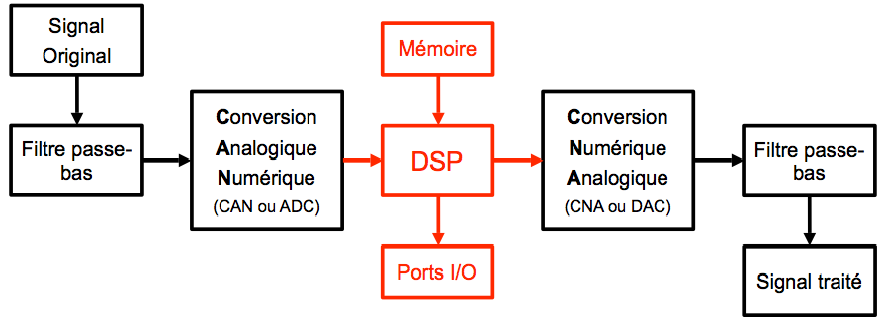
\includegraphics[scale=0.5]{EssaiImage.png}
\captionof{figure}{Chaîne typique de traitements du signal \cite{ImageChaineTrait}}
\end{center}
On y remarque que minimalement, un système de traitement complet devra contenir des éléments qui réalisent ces $ 5 $ étapes. A l'arrivée du signal il sera d'abord adapté au système, d'où le filtre anti-repliement. Ensuite, comme le traitement est numérique, il sera converti sous forme binaire par le Convertisseur Analogique-Numérique. Par après il subira un traitement adéquat (le filtrage numérique pour notre cas), puis la reconversion sous forme analogique grâce au convertisseur Numérique-Analogique. Finalement, on terminera la mise en forme du signal en le lissant grâce au filtre de lissage.
\subsection{Filtre anti-repliement}
\paragraph{}
Le filtre anti-repliement est nécessaire pour faire respecter le théorème de Shannon; il évite le repliement de spectre auquel on assiste normalement si la condition de Nyquist-Shannon est violée par sous-échantillonnage (c'est-à-dire si la fréquence d'échantillonnage est inférieure au double de la fréquence maximale du signal échantillonné). Ce phénomène est pourtant de règle et n'est en rien une exception vu que normalement, les signaux réels ne sont jamais, stricto sensu, à support fréquentiel borné. Donc, les spectres réels s'étendent toujours jusqu'à l'infini (l'amplitude du signal tendant bien sûr vers $ 0 $ sans jamais s'annuler). Par conséquent, la condition de Nyquist-Shannon ne peut jamais être strictement respectée pour un signal réel. D'où l'importance d'un filtre anti-repliement.\\
Le filtre n'est en effet qu'un passe-bas permettant de limiter la fréquence maximale prise par le signal à traiter pour que nous soyons sûr de choisir une fréquence d'échantillonnage valable (valeur non infinie).\\
Les figures \ref{NonRepliement} et \ref{OuiRepliement} nous présentent de façon imagées le répliement et l'absence de repliement.\newpage
\begin{center}
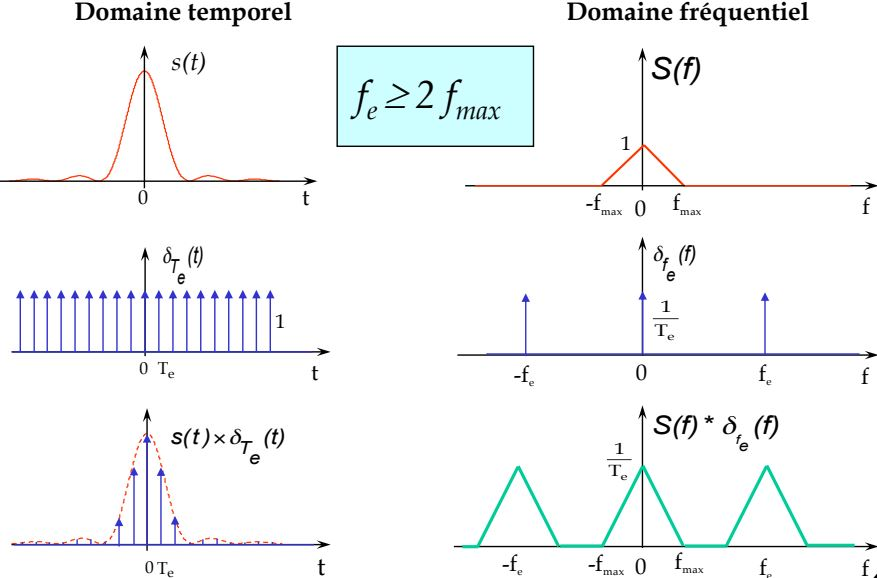
\includegraphics[scale=0.5]{nonReplie.jpg}
\captionof{figure}{Absence de repliement\cite{Tds}}\label{NonRepliement}
\end{center}
\begin{center}
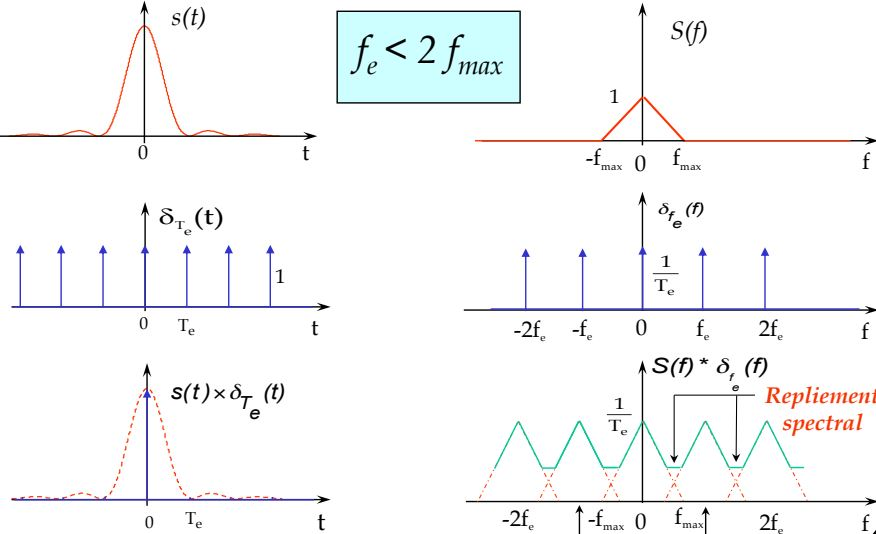
\includegraphics[scale=0.5]{Replie.jpg}
\captionof{figure}{Présence de repliement\cite{Tds}}\label{OuiRepliement}
\end{center}
\paragraph{}
Il est donc indispensable d'intercaler un filtre anti-repliement avant le convertisseur permettant le passage de l'analogique au numérique. C'est un filtre analogique passe-bas de fréquence de coupure $ Fe / 2 $ (dans l'idéal).\\
En pratique, le filtre passe-bas parfait n'existe pas et le repliement du filtre numérique $ f > \dfrac{Fe}{2}  $ est partiellement éliminé. La qualité se paie par l'utilisation d'un filtre anti-repliement élaboré (ordre élevé) \cite{20Filtr}.\\
Ce filtre passe-bas doit avoir les caractéristiques suivantes \cite{Ponge}:
\begin{itemize}
\item[-] Fréquence de coupure égale à $ F_{max} $;
\item[-] Variations de gain minimales dans la bande passante ;
\item[-] Pente la plus raide possible après la coupure (Ordre élevé);
\item[-] Atténuation hors bande passante adaptée au nombre de bits $ n $ de la numérisation.
\end{itemize}
En effet, les signaux parasites au-delà de $ F_{max} $ vont être atténués par le filtre anti-repliement et se retrouver dans la bande du signal. Pour que ces parasites repliés ne soient pas gênant, il suffit que leur niveau soit suffisamment faible c'est à dire d'un niveau inférieur à la résolution du convertisseur analogique-numérique.\\
En conclusion, le filtre anti-repliement ne supprime pas le phénomène de repliement, mais
atténue le signal replié au point de le rendre négligeable. 
\subsection{Convertisseurs Analogique-Numérique et Numérique-Analogique}
\paragraph{}
Depuis une trentaine d'années, le traitement numérique des données prend le pas sur les
approches purement analogiques. Le recours au numérique permet en effet un stockage aisé
de l'information, une excellente reproductibilité des traitements, la possibilité de développer
relativement aisément des fonctionnalités complexes, une réduction des coûts de production, etc.\\ 
L'interface nécessaire entre le monde analogique et un traitement numérique donné est réalisé
par des convertisseurs analogique–numérique (\emph{CAN}, ou \emph{ADC} pour \emph{Analog to Digital
Converter} en anglais) et numérique–analogique (\emph{CNA}, ou \emph{DAC} pour \emph{Digital to Analog
Converter}). Le rôle d'un \emph{CAN} est de convertir un signal analogique en un signal numérique
pouvant être traité par une logique numérique, et le rôle d'un \emph{CNA} est de reconvertir le signal
numérique une fois traité en un signal analogique \cite{CoursConv}.
\paragraph{}
Pour réaliser la \emph{conversion analogique-numérique}, trois opérations sont nécessaires. Il s'agit, par ordre d'apparition, de l'échantillonnage, de la quantification et du codage. L'échantillonnage du signal doit être fait en tâchant de respecter le théorème de Shannon.Le processus est clairement illustré grâce à la figure qui suit:\newpage
\begin{center}
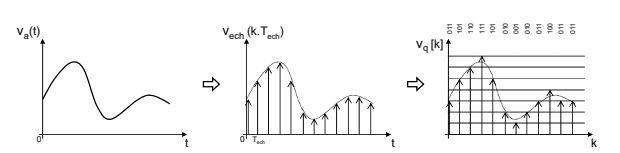
\includegraphics[scale=1]{Ech-Quant-Cod.jpg}
\captionof{figure}{Echantillonnage-Quantification-Codage \cite{CoursConv}}
\end{center}
On distingue deux grandes familles de CAN basées sur deux approches différentes du processus d'échantillonnage : les \emph{CAN classiques} dont la fréquence d'échantillonnage est telle que le
spectre du signal converti occupe quasiment toute la bande de Nyquist (Nyquist Rate ADC) et
les CAN à sur-échantillonnage (Oversampling ADC) dont seule une partie réduite du bruit de
quantification (erreur de quantification) affecte le signal converti \cite{CoursConv}.\\
Si la fréquence d'échantillonnage est bien choisie, la seule erreur introduite au cours du processus de
numérisation résulte de l'approximation faite en codant un nombre infini de valeurs analogiques par un
nombre fini $ 2^{n} $ de niveaux binaires. Le numérique n'est donc évidemment pas parfait, seulement on peut, en augmentant le nombre de bits $ n $, diminuer autant qu'on veut l'erreur introduite par la
numérisation. Avec , comme objectif, de maintenir l'erreur de quantification en dessous du seuil
de sensibilité de l'oreille humaine. Plus le nombre de bits augmente, plus le rapport signal sur bruit \emph{SNR} s'améliore \cite{Ponge}.\\
Après cette transformation, les données se dirigent vers un processeur de traitement numérique. Un traitement fait en virgule fixe est de toute évidence la plus indiquée pour être plus optimal. Il doit être considéré en cas d'implantation des algorithmes sur DSP vu que les ressources sont limitées.
\paragraph{}
Le convertisseur numérique-analogique permet de communiquer d'un système numérique vers un système
analogique. Il convertit donc un nombre binaire en une tension (ou un courant) qui lui est proportionnel.\\ L'entrée est numérique et se note formellement $ N = (b_{n-1}…b_{1}b_{0})_{2} $ avec les $ b_{i} \in \lbrace 0,1\rbrace $, $ N $ l'entrée numérique et $ n $ la résolution numérique (nombre de bits). La sortie est analogique et dans un premier temps, la conversion analogique-numérique se fait simplement par $ u_{S} = Nq + u_{S_{min}} $ avec $ u_{S} $ la tension à la sortie du convertisseur et $ q $ le \emph{ quantum ou résolution analogique} (en Volts) \cite{20Electro}.\\
Par ce qui précède on aura de toute évidence une sortie discrète du fait que les conversions sont réalisées à chaque arrivée d'un échantillon. Pour pallier à cela, le CNA a un système permettant le maintient de la tension $ u_{S} $ en sa sortie, jusqu'à l'arrivée d'un nouvel échantillon. On obtient alors en sortie, un \emph{signal analogique en escalier}. Il a ainsi un spectre fréquentiel comportant des fréquences supérieures à la fréquence maximale du signal de base. Cela est dû aux changements brusques observées pour une forme en escaliers. Il est par conséquent important de \emph{lisser} ce signal en supprimant les composantes de fréquence élevée pour obtenir finalement un signal à variations majoritairement moins brusques et/ou plus proche du signal analogique désiré.
\subsection{Filtre de lissage}
C'est le dernier élément de la chaîne de traitement du signal. Comme dit dans la section précédente, il permet de lisser le signal en escalier qu'on obtient à la sortie du CNA. Le lissage se fait par suppression des fréquences supérieures à la fréquence maximale du signal d'entrée (moitié de la fréquence d'échantillonnage). Il s'agira donc d'un filtre passe-bas comme pour le premier élément de la chaîne (filtre anti-repliement). On en illustre l'importance grâce aux figures qui suivent \cite{CoursConv} :
\begin{center}
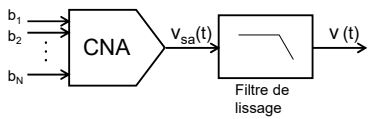
\includegraphics[scale=1]{FiltreLissage.jpg}
\captionof{figure}{Positionnement du filtre de lissage}
\end{center}
\begin{center}
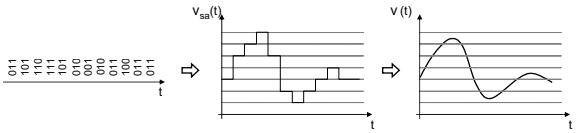
\includegraphics[scale=1]{Lissage.jpg}
\captionof{figure}{Processus complet de conversion N/A (signaux associés)}
\end{center}\newpage
\subsection{Traitement}
\paragraph{}
Une fois les données numérisées, elles sont finalement traitées. Le traitement se passe dans un processeur de traitement numérique. Il existe une multitude de processeurs, et également un grand nombre d'architectures utilisées. Néanmoins, certains processeurs sont optimisés pour le traitement du signal. Il s'agit des \emph{\textbf{DSP}} (\emph{Digital Signal Procesing}) dont on a sommairement parlé dans les parties précédentes.
\paragraph{}
Le \emph{DSP} est un microprocesseur optimisé pour exécuter des applications de traitement numérique du signal (filtrage, extraction des signaux, etc.) le plus rapidement possible. Ils sont utilisés dans la plupart des applications du traitement numérique du signal en temps réel. On les retrouve ainsi dans les modems, les téléphones mobiles, les appareils multimédia, les récepteurs GPS, les chaînes de traitement de son,... En bref, partout où l'on reçoit un signal complexe que l'on doit modifier à l'aide du filtrage. Un \emph{DSP} fournit des instructions usuelles comme la multiplication, l'addition, la soustraction, etc. Mais son jeu d'instructions est élaboré de manière à exécuter des opérations très courantes dans des algorithmes de traitement du signal les plus usuels \cite{ImageChaineTrait}.\\
Des nombreux algorithmes de traitement du signal ont par exemple besoin d'effectuer rapidement des multiplications suivies d'une addition. Les \emph{DSP} accélèrent ces genres de calcul en fournissant des instructions capables de multiplier deux nombres et d'en additionner un troisième en une seule fois (en un cycle d'horloge). Certains \emph{DSP} arrivent même à réaliser plusieurs opérations complexes de ce genre en un seul cycle d'horloge.\\
La majorité des \emph{DSP} calculent exclusivement avec des nombres à virgule fixe. L'absence d'unité en nombre flottant rend le composant meilleur marché tout en permettant une grande vitesse de traitement des données. Certains \emph{DSP} possèdent cependant des unités de calcul en virgule flottante pour des applications exigeant une large dynamique des valeurs ou une grande précision relative des résultats. Ils peuvent être combinés avec d'autres composants dans le même boîtier. C'est ainsi par exemple qu'on a, dans un même, le \emph{DSP} et les convertisseurs (\emph{Convertisseur Analogique-Numérique} et \emph{Numérique-Analogique}). \emph{Dans un appareil équipé d'un DSP, la vitesse d'exécution des calculs dans ce dernier est généralement la partie déterminante de la vitesse d'exécution du travail effectué par la machine \cite{WikiDSP}.}\newpage
\paragraph{}
Au vu de ce que nous venons de montrer dans le paragraphe précédent, le \emph{DSP} est la solution indiquée pour un système embarqué complet. Pour notre cas, sachant que nos ordinateurs sont équipés des processeurs assez rapides qui arrivent à réaliser le traitement des données avec une vitesse suffisante pour que nous testions de fonctionnement réel de notre système, nous réaliserons \emph{dans un premier temps} notre système en nous servant de l'ordinateur. Les caractéristiques utiles de ce dernier sont précisées dans la section traitant de l'élaboration de l'algorithme.\\
Il s'avère alors indubitable que, comme le traitement que nous mettons au point est un filtrage, avec comme objectif l'annulation d'écho sonore, cette partie (le traitement) suffit pour tirer des conclusions pertinentes sur le système et pour envisager (projet à long terme selon la demande ou le besoin) finalement une production du matériel conçu selon ce travail. Donc, le filtre anti-repliement et autres éléments de la chaîne de traitement du signal ne seront pas conçus par nous mais nous nous servirons de ceux de la carte son  de l'ordinateur (pour le test du fonctionnement) et ceux qui seraient couplés au boîtier du DSP (en cas de production matérielle).\\
\section{Élaboration de l'algorithme et présentation du système}
Nous allons réaliser l'annulation d'écho par utilisation de l'algorithme \emph{BPNLMS++}; les coefficients seront donc réinitialisés selon le principe illustré par les formules \ref{BPNLMS++2} et \ref{BPNLMS++1}\\
Avec $ S_{k} $ et $ S_{-k} $ définis respectivement par \\$ S_{k} = $\(\begin{pmatrix}
s(kN-p+1) & s(kN-p+2) & \cdots & s(kN+N-1)
\end{pmatrix}\)$ ^{T} $  et\\ $ S_{-k} = $\(\begin{pmatrix}
s(kN+N-1) & s(kN+N-2) & \cdots & s(kN-p+1)
\end{pmatrix}\)$ ^{T} $.\\
Les deux sont tous de longueur $ N+p-1 $ prenant directement en compte la longueur $ p $ du filtre ainsi que la taille $ N $ des blocs d'échantillons.\\
Ce qui précède nous fait immédiatement remarquer que les deux vecteurs ont les mêmes termes mais arrangés en ordre inverse. Mathématiquement, ça correspond à dire que $ S_{-k} $ s'obtient en \emph{multipliant $ S_{k} $ par une matrice carrée de dimensions adéquates et dont tous les termes sont nuls sauf la diagonale secondaire qui sera totalement constituée des $ 1 $.}\newpage
\subsection{Élaboration de l'algorithme d'apprentissage}\label{Etapes}
Soit à utiliser un processeur à $ 16 $ \emph{bits}, ce qui correspond au dernier nombre premier de Fermat, le cinquième pour être exact. En effet, si nous choisissons $ b=16 $, ça veut dire que dans la forme canonique des nombres de Fermat introduits à la sous-section \ref{NbrFermat} nous avons que $ t=4 $, soit donc que le nombre de Fermat en question est $ 2^{2^{4}}+1 = 2^{16}+1 = 65537 = F_{4}$ . Ce choix est judicieux vu que nous comptons faciliter les calculs par transformée en nombres de Fermat (FNT), car là on a bel et bien un nombre de Fermat valable (un nombre premier en l'occurrence et en plus le plus grand nombre premier de Fermat connu).\\
Aussi, étant donné ce que nous avons considéré à la sous-section \ref{MetALPHA}, entre autres les définitions selon lesquelles $ M = 2^{t+1-i} $ et $ \langle\alpha = 2^{2^{i}}\rangle_{F_{t}} $, en choisissant par exemple $ i=-2 $ on obtient une longueur de transformation $ M=128 $ et $ \langle\alpha = \sqrt[4]{2}\rangle_{F_{4}} = 4938 $.\\
Voulant conserver le fait selon lequel on ne peut pas transformer une séquence de longueur supérieure à la longueur $ M $ de la transformée, nous devons faire remarquer que vu que $ S_{k} $ et $ S_{-k} $ sont de longueur $ N+p-1 $, on doit impérativement respecter la condition $ M\geq N+p-1 $ ou alors prendre $ N+p-1 < M $ pour le compléter ensuite jusqu'à la longueur $ M $. Alors, pour choix on peut prendre par exemple $ N=64 $ et $ p=64 $ (deux moitiés de $ M $). Sur base de cela, nous aurons les étapes de l'algorithme :
\begin{itemize}
\item[1°)] \textbf{Acquisition et préparation du signal à manipuler;}\\
\item[2°)] \textbf{Écriture des fonctions qui réalisent la FNT et son inverse}\\
Après extraction du signal, nous pourrons être amenés à effectuer une transformée en nombres de Fermat sur le vecteur constitué des échantillons. Pour cela, nous devons réaliser ce qui suit:
\begin{itemize}
\item[1.] Fonction réalisant la transformée de la séquence de longueur fixée $ M $;
\item[2.] Fonction réalisant la transformée inverse d'une séquence de longueur identique;
\end{itemize}\newpage
\item[3°)] \textbf{Écriture d'une boucle devant réaliser l'apprentissage (adaptation du filtre) :}
\begin{itemize}
\item[1.] Fenêtrage d'un bloc de $ 64 $ échantillons du signal d'entrée;
\item[2.] Construction globale du signal d'entrée à considérer $ S_{k} $ en faisant précéder les $ 64 $ échantillons de $ p-1 $ derniers échantillons provenant du signal $ S_{k-1} $;
\item[3.] Vu qu'ainsi on a $ S_{k} $ de longueur $ M=128 $ termes en le complétant, calcul de sa FNT par appel de la procédure correspondante;
\item[4.] Initialisation des coefficients du filtre (comme notre filtre est de longueur $ p=64 $, nous prendrons pour filtre initial, un filtre dont tous les $ 64 $ termes sont tous nuls);
\item[5.] Complément des coefficients du filtre par des 0 par ajout de $ M-p $ termes nuls pour obtenir un vecteur pouvant subir une FNT de longueur $ M $;
\item[6.] Calcul de la FNT du vecteur ainsi formé par appel de la procédure correspondante;
\item[7.] Calcul du produit terme à terme de ces deux FNT précédemment obtenus (Transformée de $ W_{k} $ complété multipliée par la transformée de $ S_{k} $;
\item[8.] Calcul de la FNT inverse du produit obtenu par appel de la procédure dédiée (cela donne le produit de convolution des coefficients du filtre par le signal d'entrée. Donc on obtient $ y_{w_{k}} $ dont seuls les $ N $ derniers termes correspondent aux $ N $ vrais échantillons formant $ y_{w_{k}} $;
\item[9.] Formatage de $ y_{w_{k}} $ par élimination des $ M-N $ premiers termes inutiles. Pour cela, on multiplie une matrice de taille $ N\times M $ dont les $ M-N $ premiers termes de chaque ligne sont tous nuls et l'autre partie est semblable à une matrice unitaire de taille $ N $ (c'est-à-dire que tous ses termes diagonaux sont égaux à $ 1 $) par le vecteur $ y_{w_{k}} $ obtenu après la transformation inverse de l'étape précédente ; on obtient après cette multiplication, une matrice $ N\times 1 $ qui correspond effectivement au vrai vecteur $ y_{w_{k}} $ recherché;
\item[10.] Calcul du vecteur d'erreur par comparaison (une différence) de la valeur trouvée $ y_{w_{k}} $ avec la valeur désirée $ y_{k} $;
\item[11.] Complément de ce vecteur par des 0 jusqu'à obtenir un vecteur de longueur $ M $ car c'est bien cela la longueur de la transformée que nous avons choisi d'utiliser (on aura ajouté alors $ M-N $ termes nuls);
\item[12.] Calcul de la FNT du vecteur d'erreur ainsi complété;
\item[13.] Construction du vecteur image $ S_{-k} $ en multipliant le vecteur $ S_{k} $ déjà bien formaté et complété par une matrice de taille $ M $ (matrice carrée donc) dont tous les termes sont nuls à part ceux de la diagonale secondaire qui sont tous égaux à $ 1 $. La multiplication de cette dernière matrice par $ S_{k} $ a donc pour effet de renverser l'ordre de ses termes;
\item[14.] Calcul de la FNT de ce vecteur image;
\item[15.] Calcul du produit terme à terme de ce vecteur image transformé avec le vecteur d'erreur transformé;
\item[16.] Calcul de la transformée inverse du résultat ainsi obtenu (la réponse correspond au vecteur $ \varepsilon_{k}\ast S_{-k} $ dont seuls les $ p $ derniers termes forment le vrai vecteur recherché;
\item[17.] Formatage du résultat obtenu en lui appliquant une matrice que nous nommons $ E $, de dimension $ p\times M $ pour obtenir au final un vecteur de taille $ p $. Pour cela on multiplie la matrice construite $ E $ par le résultat obtenu à l'étape précédente. Cette matrice en est en fait une dont les $ M-p $ premiers termes de chaque ligne sont nuls et l'autre partie est comme une matrice carré de taille $ p\times p $ dont les termes de la diagonale principale sont tous égaux à $ 1 $ et les autres sont tous nuls (matrice unitaire de taille $ p $);
\item[18.] Calcul du produit terme à terme du vecteur d'entrée $ S_{k} $ transformé  avec son vecteur image $ S_{-k} $ aussi transformé;
\item[19.] Calcul de la transformée inverse du précédent produit (cela nous permet d'obtenir la fonction d'autocorrélation du signal d'entrée $ R_{ss}(k) = S_{k}\ast S_{-k} $ qui est aussi réduit à ses $ p $ derniers termes en lui appliquant la matrice $ E $ comme cela a été fait à l'étape $ 17 $;
\item[20.] Construction de la matrice diagonale $ G_{k} $ de taille $ p\times p $ tel qu'elle fut définie à la sous-section \ref{MatrGk};
\item[21.] Calcul des vecteurs $ G_{k}.(\varepsilon_{k}\ast S_{-k}) $ et $ G_{k}.R_{ss}(k) $;
\item[22.] Réinitialisation des coefficients du filtre en appliquant l'algorithme \emph{BNLMS} (tout en tenant compte de la dernière remarque de sur l'état formel des formules du \emph{BNLMS} et du \emph{BPNLMS}). On appliquera donc précisément \\
 \\
\begin{center}
$ W_{k+1}(i)=W_{k}(i)+\frac{\lambda}{[R_{ss}(k)](i)+\beta}[(\varepsilon_{k}\ast S_{-k})](i) $
\end{center};
\item[23.] Réinitialisation des coefficients du filtre en appliquant l'algorithme \emph{BPNLMS} en tenant également compte du fait que la formule s'exprime réellement par :\\
 \\
\begin{center}
$ W_{k+1}(i)=W_{k}(i)+\frac{\lambda}{[G_{k}R_{ss}(k)](i)+\beta}[G_{k}(\varepsilon_{k}\ast S_{-k})](i) $
\end{center};
\item[24.] Construction du vrai vecteur des coefficients du filtre en prenant tous les termes impairs égaux aux termes impaires correspondants du vecteur trouvé à l'étape précédente et les termes pairs aux termes pairs correspondant du vecteur trouvé à l'étape $ 22 $ (ainsi on vient de réinitialiser le filtre en appliquant le \emph{BPNLMS++});
\item[25.] Relance de la boucle jusqu'au nombre d'itérations voulu.
\end{itemize}
\item[4°)] \textbf{Fin de la boucle, renvoi des valeurs figées des coefficients du filtre en les formatant si nécessaire}\\
\end{itemize}
\subsection{Présentation du système réel}
Après cette étape d'apprentissage, on obtiendra les coefficients du filtre qui modélisent au mieux la réponse impulsionnelle de l'enceinte considérée. Ainsi, comme mentionné à la sous-section \ref{Convol}, le signal d'écho obtenu dans l'enceinte considérée peut bel et bien aussi s'obtenir,dans les mêmes conditions, par convolution du signal d'entrée avec le vecteur formé des coefficients du filtre ainsi construit. Cette solution est cruciale et déterminante pour l'efficacité et la rapidité\footnote{Sans ignorer les autres avantage d'un système d'annulation d'écho tout court.} des systèmes de communication. En effet, annuler directement l'écho grâce à un modèle numérique équivalent à l'enceinte utilisée, nous permet :
\begin{itemize}
\item[•] De ne pas avoir à empêcher un locuteur de parler lorsque l'autre parle;
\item[•] De simuler l'écho venant de n'importe quelle source (sélectionner un signal en particulier dont on veut extraire l'écho) pour ensuite le soustraire du signal qu'on compte transmettre.
\end{itemize}
Ce qui serait carrément impossible sans cette modélisation de la réponse de la salle.
\paragraph{}
Le système se résume donc ainsi :\\
Deux interlocuteurs ayant chacun un combiné de communication, équipés chacun d'un système d'annulation d'écho, sont dans deux enceintes différentes (et dans la même enceinte à la limite ; mais c'est sans intérêt). On procède premièrement à une phase d'apprentissage où, un son de quelques secondes est émis par le haut-parleur des combinés de chaque locuteur et le filtre de chaque combiné est mis à jour. Ensuite s'établit la communication entre les deux interlocuteurs où, chaque fois que l'une des sources émet un signal, on en soustrait la modélisation de l'écho du signal venant de l'autre. Ainsi, aucun des deux ne peut réentendre sa voix à travers son haut-parleur. Cela résout le problème d'écho acoustique associé au système de communication considéré.\\ Dans la suite (pour les essais) nous n'allons considérer qu'un interlocuteur.Pour cela, le signal venant de l'autre sera juste appelé \emph{signal lointain} et celui qui vient du locuteur présent dans la salle d'expérimentation sera dit \emph{signal local}. Cela nous permettra de réaliser l'adaptation du filtre et de vérifier si le filtre obtenu modélise bel et bien l'enceinte prototype.
\section{Implémentation de l'algorithme et simulations}
Dans cette section, nous allons écrire l'algorithme élaboré dans la section précédente en langage Matlab (qui a évidemment une syntaxe proche du \textbf{C} et qui nous permettra aumoins de réaliser des expérimentations de manière moins complexe).\\
Utilisant un processeur à virgule flottante (celui de l'ordinateur), nous n'allons pas nous cramponner sur le formatage du signal d'entrée. Par conséquent, la transformation de Fourier va suffire pour avoir un aperçu de l'algorithme global.
\subsection{Traitement brut des données}\label{Brut}
Ce traitement revient à réaliser l'adaptation des coefficients du filtre à la manière dont la théorie a été élaborée au début du second chapitre. Donc sans optimiser le temps de calcul avec un traitement par blocs. Nous allons donc réaliser un algorithme d'adaptation évoluant échantillon par échantillon et non par blocs. Ceci est utile pour remarquer la précision de ce traitement malgré le manque de robustesse et la charge de calcul. L'algorithme élaboré pour cet effet est ,sous \textbf{Matlab}, donné par l'annexe \ref{Anne1} .\\
La compilation de ce code a duré $ 12.424632 $ \emph{secondes} (valeur donnée par le chronomètre intégré à Matlab en excluant la prise du son) pour un signal d'entrée pris enregistré sur $ 40 $ \emph{secondes} (voir la ligne $ 12 $ de ce code) pour pouvoir pousser très loin l'adaptation (jusqu'à $ 20850 $ tours de boucle principaux comme on le voit à la ligne $ 43 $ de ce code).\\
Le signal d'entrée, avec \textit{les niveaux de son représentés en fonction des numéros d'échantillon}, était le suivant :
\begin{center}
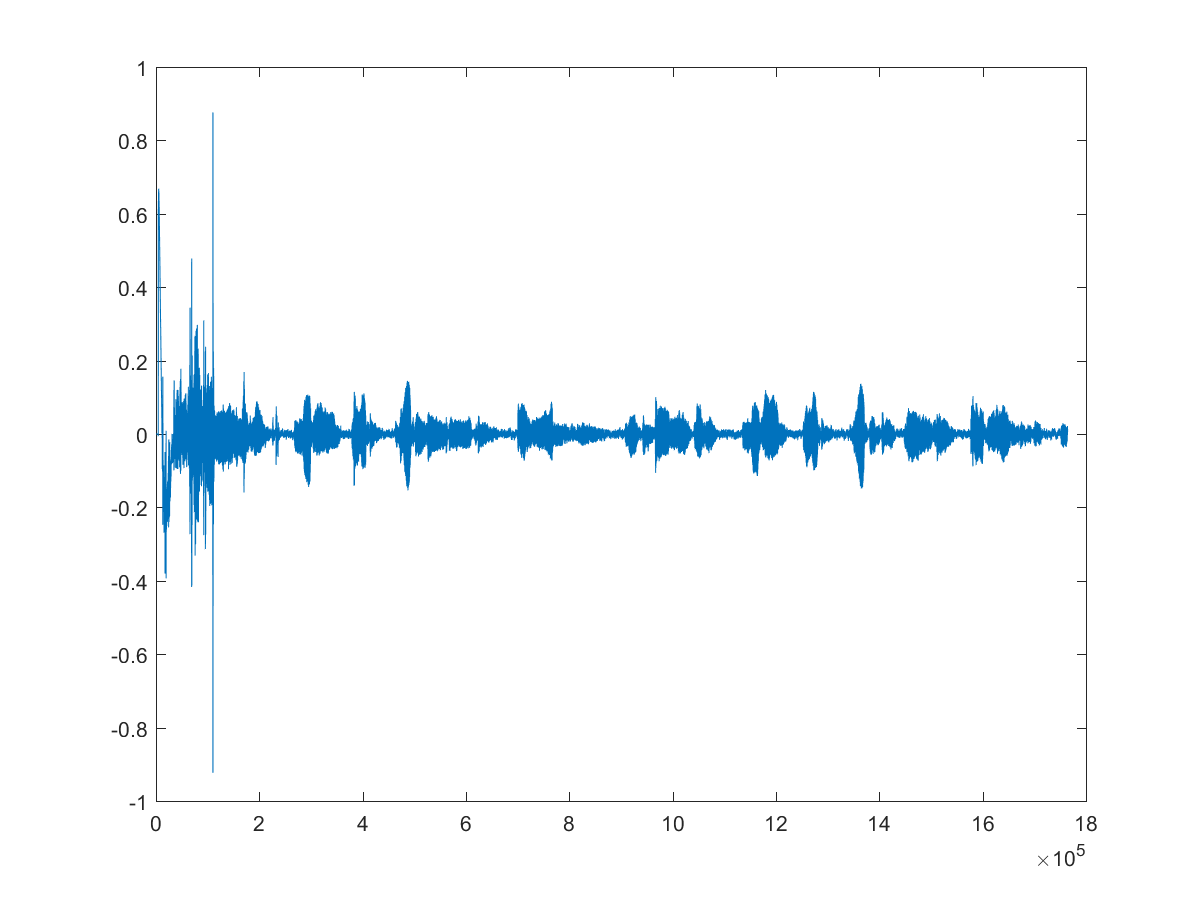
\includegraphics[scale=0.7]{Entree.png}
\captionof{figure}{Signal d'entrée utilisé}
\label{entree}
\end{center}
Le signal présenté sur la figure \ref{entree} a été obtenu en nous enregistrant pendant $ 40 $ \textit{secondes} entrain de chanter de façon arbitraire juste pour le test. Et cela a été ensuite tracé en utilisant \textit{Matlab} (voir les annexes \ref{Anne1} et \ref{Anne2}).\\
Pour $ i=20850 $ tours de boucles (voir la ligne $ 43 $ du code), nous avons obtenu \textit{les coefficients du filtre représentés en fonction des numéros d'échantillons} par: 
\begin{center}
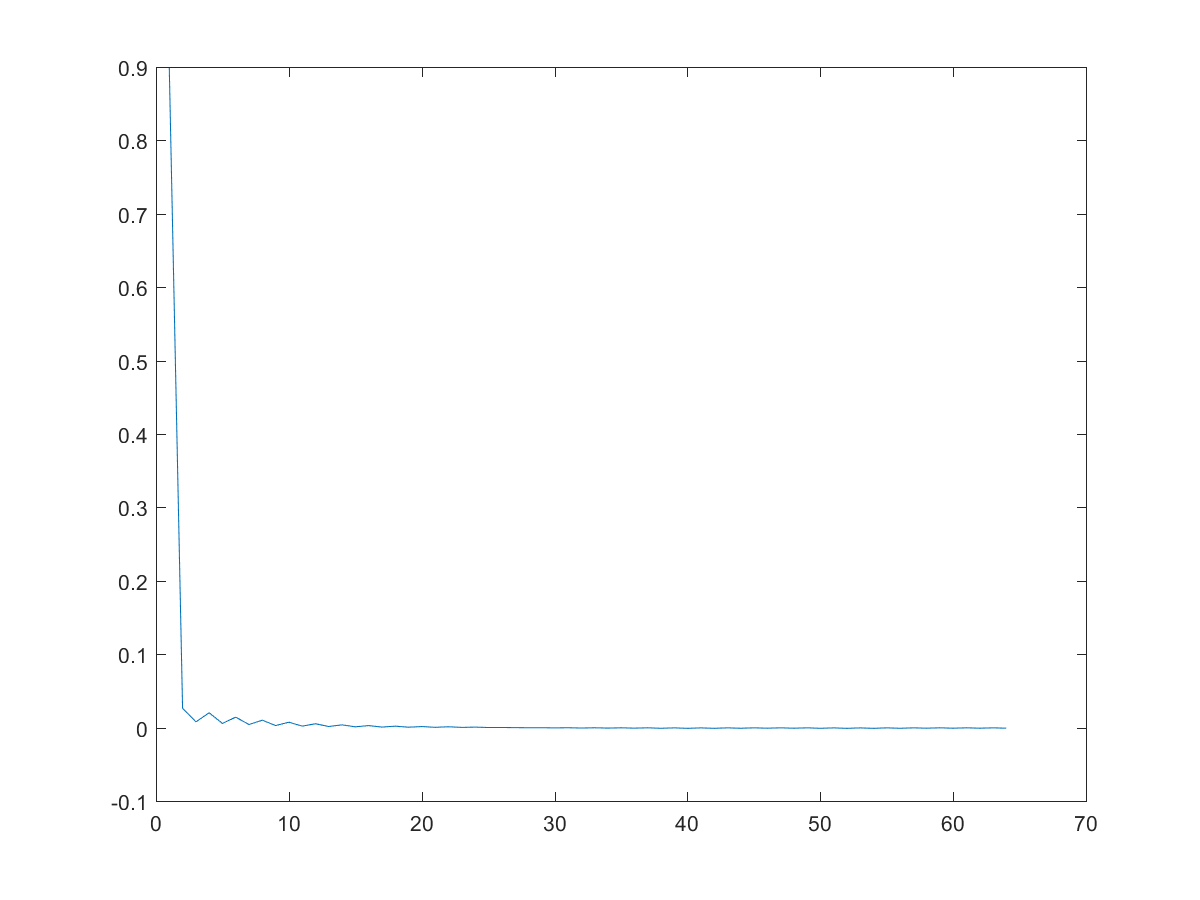
\includegraphics[scale=0.7]{Filtre1.png}
\captionof{figure}{Valeurs des $ 64 $ coefficients du filtre}
\label{f1}
\end{center}
Sous cette forme, sur la figure \ref{f1}, on a remarqué que la convergence du filtre est relativement lente bien que le résultat soit plus parfait. Cela sera plus clairement compris avec les sections qui suivent.
\subsection{Traitement par bloc des données}\label{Bloc}
L'algorithme utilisé et qui suit les étapes décrites précédemment (à la section \ref{Etapes} qui concerne l'élaboration de l'algorithme conseillé pour un implantation sur DSP) est donné à l'annexe \ref{Anne2} .\\
Il est très important de signaler que bien que les étapes décrites lors de l'élaboration textuelle de l'algorithme soient faites pour le cas d'un traitement par FNT et \emph{pour un processeur à virgule fixe fonctionnant sous $ 16 $ bits}, le fait que nous ayons utilisé un processeur sous $ 64 $ \emph{bits} et la transformée de Fourier est tout à fait admissible. L'algorithme textuel a juste été élaboré pour considérer le cas le plus général et pour nous guider dans l'implémentation, surtout que cela permet également d'optimiser à la fois les coûts et l'exploitation des ressources.\\ 
On remarque des simplifications drastiques en ce qui concerne le formatage des vecteurs. C'est ainsi qu'à la ligne $ 73 $ de ce code (annexe \ref{Anne2} ), on remarque qu'au lieu de multiplier le vecteur à $ 128 $ termes par une matrice particulière $ E $ (comme nous le suggère le point $ 3 $ en son étape $ 17 $ de la sous-section \ref{Etapes} sur les étapes de l'algorithme), \textbf{Matlab} nous permet d'extraire très simplement ces derniers termes. C'est le cas également aux lignes $ 62 $ et $ 77 $ (annexe \ref{Anne2} toujours)  où les manipulations sont grandement simplifiées par rapport à ce que nous proposions au préalable. Ces propositions ont tout de même le mérite d'être plus générales comme méthode et donc utilisables même quand le langage ne permet pas une manipulation très simple des matrices.\\
La compilation de ce code a duré $ 8.219884 $ \emph{secondes} (valeur donnée par le chronomètre intégré à Matlab en excluant la prise du son) pour le même signal d'entrée que précédemment (voir la ligne $ 12 $ de ce code et la figure \ref{entree}) pour pouvoir pousser très loin l'adaptation.\\
Ainsi on a obtenu \textit{en fonction des numéros d'échantillons le filtre} suivant:
\begin{center}
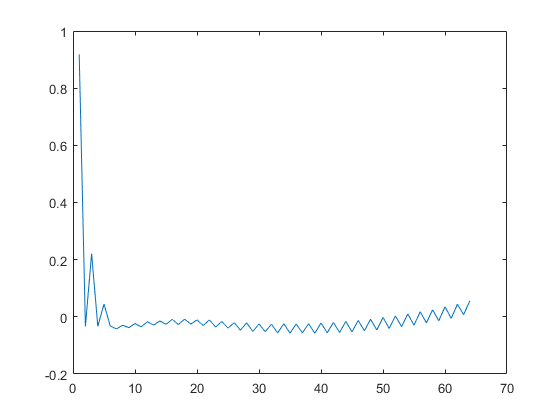
\includegraphics[scale=1]{Filtre2.png}
\captionof{figure}{Les $ 64 $ coefficients du filtre 2}
\label{f2}
\end{center}
Le filtre (ses coefficients) obtenu sur la figure \ref{f2} par contre est moins précis mais s'obtient plus vite à cause de la grande vitesse de convergence des algorithmes de traitement par bloc. Normalement, suite aux manipulations des vecteurs, on obtient un \emph{filtre renversé et décalé} comme on le voit sur cette figure:
\begin{center}
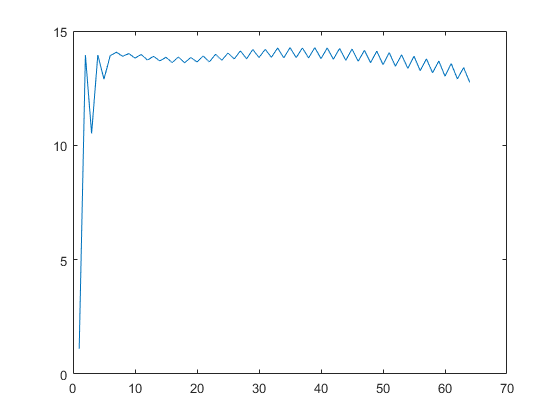
\includegraphics[scale=0.9]{Filtre2Ren.png}
\captionof{figure}{Les $ 64 $ coefficients du filtre 2 non formatés}
\label{fR}
\end{center}
De cela on obtient très aisément la courbe recherchée trouvée à la figure \ref{f2} grâce au formatage des coefficients, réalisé avec le bout de code de la ligne $ 112 $ (annexe \ref{Anne2} ) donné par:
\begin{verbatim}
w=((ones(1,64))*(mean(w))-(w))/(mean(w));
\end{verbatim}
Pour réaliser ce formatage, il suffit de détecter la valeur moyenne (on écrit \textbf{mean(w)}). Pour notre signal d'entrée, le filtre non formaté avait pour moyenne $ (13.5) $ (voir la figure \ref{fR}).
\subsection{Essais comparés}\label{essais}
Essayons, pour le même signal d'entrée (figure \ref{entree}), de trouver les coefficients du filtre pour les deux cas en considérant différentes valeurs de $ i $ (nombre d'itérations qu'on voit aux lignes $ 43 $ des codes qu'on a aux annexes \ref{Anne1} et \ref{Anne2} ) et observons l'évolution des coefficients. Nous prendrons des valeurs inférieures à $ 20850 $ car pour une boucle allant trop au delà, nous risquons de dépasser la longueur maximale des vecteurs. Notons que le signal d'entrée formaté sous forme vectorielle était de taille $ 1764352 $ échantillons.
\begin{itemize}
\item[1°)] Pour $ i=10000 $ on obtient:
\begin{center}
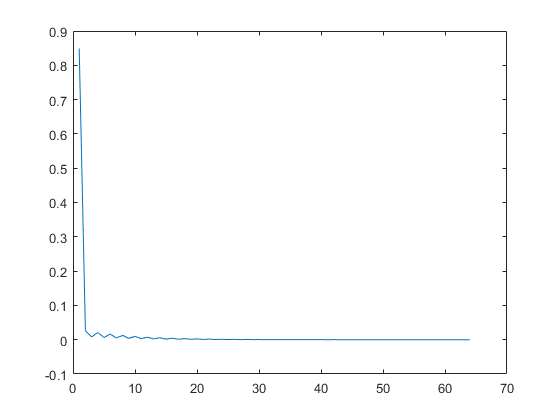
\includegraphics[scale=0.5]{Filtre1-10000.png}
\captionof{figure}{Coefficients du filtre 1 pour 10000 itérations}
\label{f1-10000}
\end{center}
Sur la figure \ref{f1-10000} on voit les coefficients du filtre, obtenus après $ i=10000 $ itérations par l'algorithme de traitement échantillon par échantillon (ce qui a duré $ 6.073958 $ secondes). On a pratiquement le bon filtre.
\begin{center}
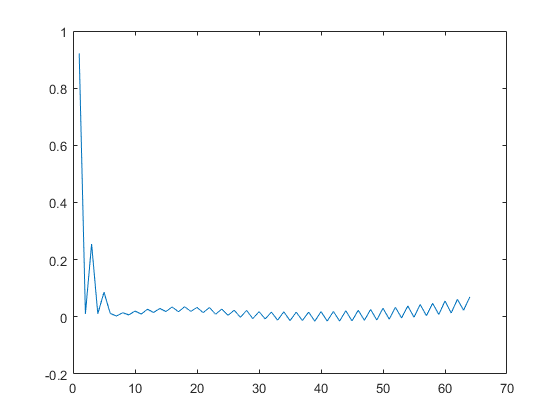
\includegraphics[scale=0.5]{Filtre2-10000.png}
\captionof{figure}{Coefficients du filtre 2 pour 10000 itérations}
\label{f2-10000}
\end{center}
Sur la figure \ref{f2-10000} on voit les coefficients du filtre, obtenus après $ i=10000 $ itérations par l'algorithme de traitement par blocs d'échantillons (ce qui a duré $ 3.920202 $ secondes, presque la moitié du temps nécessaire au traitement brut précédent).  C'est pratiquement les mêmes coefficients que ceux obtenus pour le cas où le nombre d'itérations était $ 20850 $.
\item[2°)] Pour $ i=1000 $ on obtient:
\begin{center}
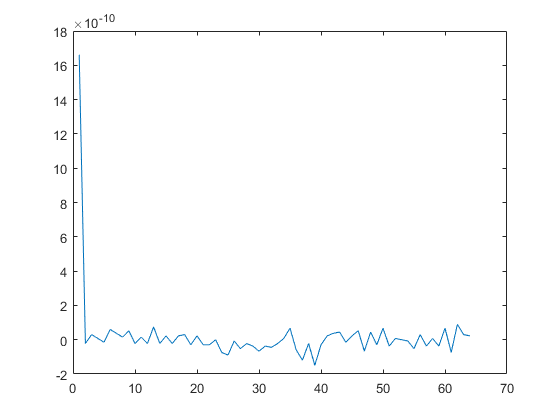
\includegraphics[scale=0.5]{Filtre1-1000.png}
\captionof{figure}{Coefficients du filtre 1 pour 1000 itérations}
\label{f1-1000}
\end{center}
Sur la figure \ref{f1-1000} on voit les coefficients du filtre, obtenus après $ i=1000 $ itérations par l'algorithme de traitement échantillon par échantillon (a duré $ 0.658588 $ secondes). Malgré que la forme est bonne, les coefficients sont très faibles.
\begin{center}
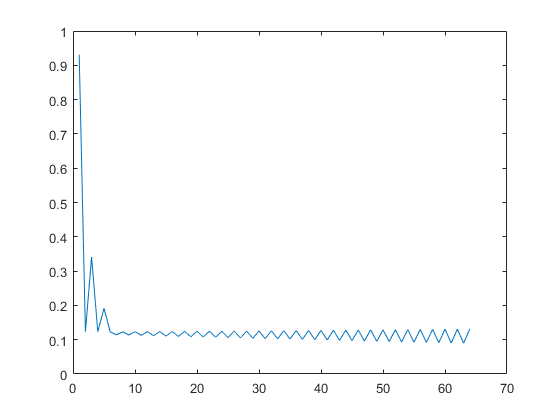
\includegraphics[scale=0.5]{Filtre2-1000.png}
\captionof{figure}{Coefficients du filtre 2 pour 1000 itérations}
\label{f2-1000}
\end{center}
Sur la figure \ref{f2-1000} on voit les coefficients du filtre, obtenus après $ i=1000 $ itérations par l'algorithme de traitement par blocs d'échantillons (pour un temps de calcul de $ 0.426955 $ secondes).  Malgré un léger décalage vers le haut, on a obtenu pratiquement le filtre final.
\item[3°)] Pour $ i=100 $ on obtient:
\begin{center}
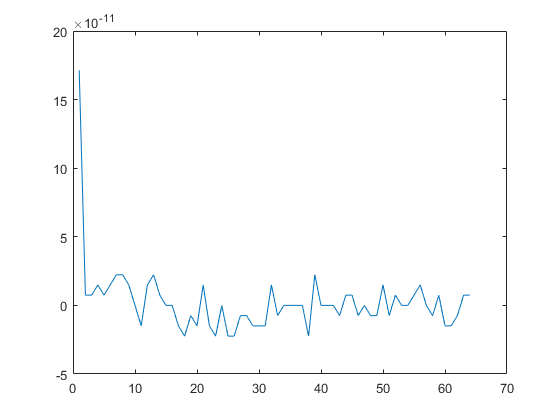
\includegraphics[scale=0.5]{Filtre1-100.png}
\captionof{figure}{Coefficients du filtre 1 pour 100 itérations}
\label{f1-100}
\end{center}
Sur la figure \ref{f1-100} on voit les coefficients, obtenus après $ i=100 $ itérations par l'algorithme de traitement échantillon par échantillon (durée de compilation de $ 0.079877 $ secondes). Malgré que la forme commence déjà à se dessiner, les coefficients sont très faibles (c'est un filtre à coefficients quasi nuls).
\begin{center}
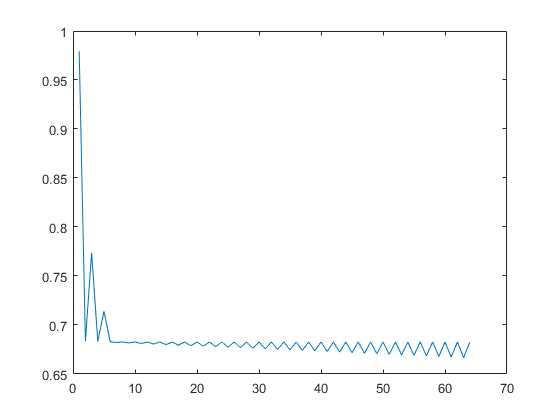
\includegraphics[scale=0.5]{Filtre2-100.png}
\captionof{figure}{Coefficients du filtre 2 pour 100 itérations}
\label{f2-100}
\end{center}
Sur la figure \ref{f2-100} on voit les coefficients du filtre, obtenus après $ i=100 $ itérations par l'algorithme de traitement par blocs d'échantillons (ce qui a duré $ 0.057885 $ secondes). La forme commence déjà à se dessiner mais les coefficients sont encore trop décalés vers le haut.
\item[4°)] Pour $ i=10 $ on obtient:
\begin{center}
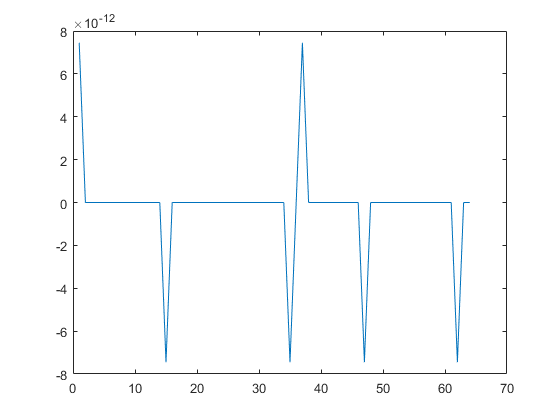
\includegraphics[scale=0.5]{Filtre1-10.png}
\captionof{figure}{Coefficients du filtre 1 pour 10 itérations}
\label{f1-10}
\end{center}
Au début de l'adaptation du filtre , les coefficients sont très mauvais. La figure \ref{f1-10} représente l'adaptation du filtre échantillon par échantillon après $ 10 $ itérations. 
\begin{center}
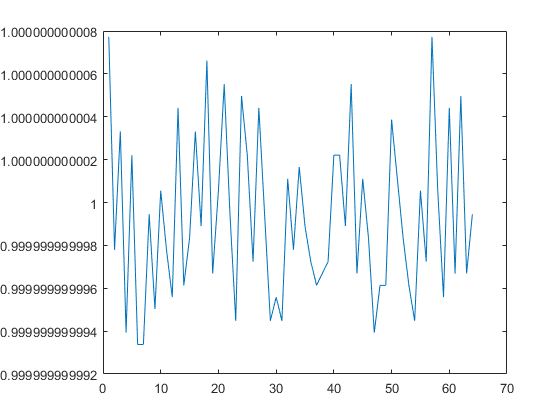
\includegraphics[scale=0.5]{Filtre2-10.png}
\captionof{figure}{Coefficients du filtre 2 pour 10 itérations}
\label{f2-10}
\end{center}
Au début de l'adaptation du filtre, les coefficients sont très mauvais. Pour $ 10 $ itérations, avec le traitement par blocs, on n'a toujours pas même l'esquisse des valeurs souhaitées, comme on peut le voir sur la figure \ref{f2-10}.
\item[4°)] Il y a également deux valeurs particulières pour les deux implémentations, les valeurs de $ i $ auxquels les filtres auront presque complètement atteint les coefficients escomptés. Après plusieurs essais on obtient:
\begin{itemize}
\item[•] $ i=4370 $ pour le filtre en traitement brut (filtre 1)
\begin{center}
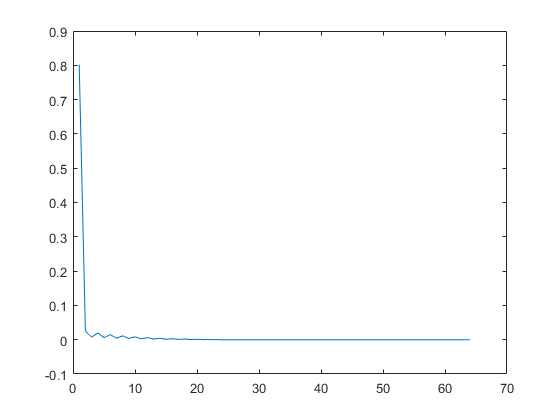
\includegraphics[scale=0.7]{Filtre1Bon.png}
\captionof{figure}{Coefficients du filtre 1 pour 4370 itérations}
\label{f1b}
\end{center}
L'algorithme de traitement échantillon par échantillon donne des très bons coefficients mais après beaucoup d'itérations ($ i=4370 $) et trop de temps ($ 3.296686 $ \emph{secondes} pour notre cas) comme on peut le voir sur la figure \ref{f1b}.
\item[•] $ i=400 $ pour celui du traitement par blocs (filtre 2)
\begin{center}
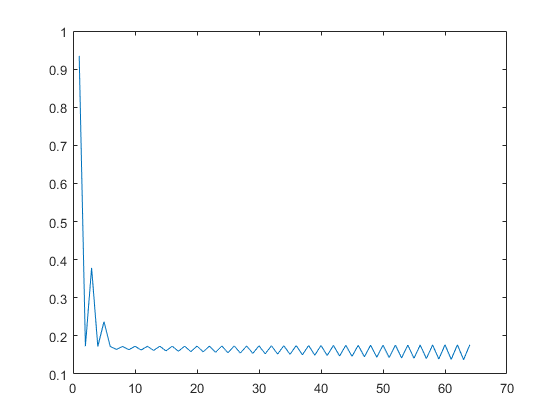
\includegraphics[scale=0.7]{Filtre2Bon.png}
\captionof{figure}{Coefficients du filtre 2 pour 400 itérations}
\label{f2b}
\end{center}
Comme on peut le voir sur la figure \ref{f1b}, l'algorithme de traitement par bloc permet d'obtenir après seulement $ 0.173829 $ \emph{secondes}, des coefficients très proches des bonnes valeurs (bien que n'étant pas très affinés, ils sont assez bons pour que le passage du signal à travers un filtre ayant des telles valeurs nous donne presqu'exactement la sortie souhaitée).
\end{itemize}
\end{itemize}
\section{Analyse des résultats et explication de l'implantation sur DSP}
\subsection{Analyse des résultats}
Ce que nous venons d'obtenir à la sous-section \ref{essais} est très crucial pour remarquer la puissance du traitement par blocs. On remarque très bien que le filtre élaboré par un traitement échantillon par échantillon n'évolue pas très vite vers les vraies valeurs, et se dégrade très vite avec la réduction du nombre d'itérations, tandis que le traitement par blocs est à la fois rapide (en terme de temps de calcul) et converge plus vite vers le filtre optimal.\\
\emph{Dans le code , à la ligne $ 61 $ pour le premier (annexe \ref{Anne1} ) et $ 64 $ (annexe \ref{Anne2} ) pour le second, on a spécifié que le résultat attendu à la sortie du filtre devait être, pour tester le fonctionnement de notre algorithme, le même signal mis à l'entrée (donc l'erreur est minimisée de manière à ce que le signal d'entrée soit le même que celui obtenu après avoir traversé le filtre). Or nous savons très bien que pour avoir une sortie identique à l'entrée, la réponse impulsionnelle du filtre doit être une impulsion toujours. Et évidemment, le filtre optimal que nous avons obtenu s'approche d'une impulsion comme on le voit très bien aux figures \ref{f1} et \ref{f2}.} \textbf{Le premier est évidemment plus proche d'une impulsion que le second bien qu'obtenu grâce à un algorithme moins robuste}. En effet, le premier algorithme, qui nous permet d'obtenir des meilleurs coefficients, converge très lentement et se dégrade très vite quand on diminue le nombre d'itérations; en plus il prend trop de temps pour donner les résultats. Pour s'en convaincre, voir les figures \ref{f1-10000} puis \ref{f1-1000} ensuite \ref{f1-100} et finalement \ref{f1-10}, on remarque très bien dans peu de temps que l'amplitude des coefficients du filtre se dégrade très vite et que les coefficients eux aussi deviennent de plus en plus écartés des bonnes valeurs jusqu'à la dégradation complète à la dernière figure, la figure \ref{f1-10}). Le second, celui obtenu grâce à l'algorithme de traitement par blocs et dont l'évolution des coefficients est représentée en ordre par les figures \ref{f2-10000} puis \ref{f2-1000} ensuite \ref{f2-100} et finalement \ref{f2-10}, est moins précis mais nettement plus robuste que le premier. En effet, il demande peu de temps de calcul et se dégrade très lentement quand on diminue le nombre d'itérations. \emph{Malheureusement, il nécessite d'importantes corrections d'erreurs.}\\
En bref, la comparaison des résultats représentés par les figures \ref{f1b} et \ref{f2b} nous montre nettement la supériorité du traitement par blocs par rapport au traitement échantillon par échantillon. On remarque très clairement la nécessité d'une implantation par blocs pour avoir un traitement en temps réel (voir les commentaires afférentes aux deux figures précédentes). 
\subsection{Explication de l'implantation sur DSP}
L'implantation sur DSP à virgule fixe et sous $ 16 $ \emph{bits} exige l'adaptation de l'algorithme élaboré (celui de l'annexe \ref{Anne2} ) de manière à ce qu'on puisse réaliser le même traitement. Pour cela, on n'a que deux choses particulières à réaliser:
\begin{itemize}
\item Formater le signal d'entrée de manière à l'adapter au processeur si nécessaire et
\item Ecrire une fonction qui réalise la transformée en nombres de Fermat tel qu'on l'a décrite et opltimisé dans les parties précédentes ainsi que son inverse. En utilisant juste les formules données.
\end{itemize}
Après avoir réalisé cela, le code sera exactement le même que celui qui a été élaboré pour le traitement par blocs en se basant sur l'esquisse qui a été faite de l'algorithme au point \ref{Etapes}. Le formatage quant à lui, quand il est nécessaire, se réalise facilement par des manipulations simples (multiplications suivies des arrondissements). Cette dernière méthode introduit évidemment une erreur mais dès qu'on envisage de l'utiliser, on peut \emph{étudier la technique adaptée pour la réduction de l'erreur qui serait introduite à la fois par ce formatage et celui réalisé durant le filtrage}. Après avoir ainsi adapté l'algorithme, il faudra alors l'écrire en \emph{assembleur} pour adapter le code à l'architecture du DSP choisi ou carrément en langage \emph{C}, laissant au compilateur le soin d'optimiser le code en l'adaptant au DSP (C'est la solution la plus simple en fait).\newpage
\section{Annulation d'écho}
Notre travail a consisté principalement à élaborer le filtre qui peut s'utiliser pour annuler l'écho dans un système de communication. Nous allons montrer la meilleure annulation que nous avons pu obtenir avec les filtres conçus. Il s'agit de l'annulation grâce au filtre implémenté par l'algorithme en annexe \ref{Anne1} qui est le plus précis (l'autre est le plus indiqué en cas d'embarquement mais nécessite d'astucieuses corrections d'erreurs). Les coefficients de ce filtre sont donnés par la figure \ref{f1}, il correspond presqu'exactement à une impulsion. On obtient d'abord la sortie et l'annulation par le code \emph{Matlab} suivant\footnote{Se référer à l'annexe \ref{Anne1} pour remarquer que \emph{myrecording} représente le signal en entrée}:
\begin{verbatim}
1-	sortie=conv(w,myrecordings);
2-	echoTransmis=(sortie(1:1608500))-(myrecordings(1:1608500));
\end{verbatim}
Ce bout de code a été exécuté à part, mais après l'exécution de celui d'adaptation pour pouvoir utiliser les mêmes variables. Il réalise en sa première ligne, la convolution du vecteur formé par les coefficients du filtre avec le signal d'entrée (c'est le filtrage si on pose que le filtre est approximativement linéaire). A la deuxième ligne on réalise alors la suppression d'écho pour le cas où le signal n'est pas trop modifié par l'enceinte (comme nous l'avons posé pour tester la validité de nos codes). On a considéré $ 1608500 $ échantillons pour ne pas risquer de dépasser la taille totale des vecteurs car le signal en entrée avait environs $ 1700000 $ échantillons.
\begin{figure}[!h]
\begin{subfigure}{.5 \textwidth}
\centering
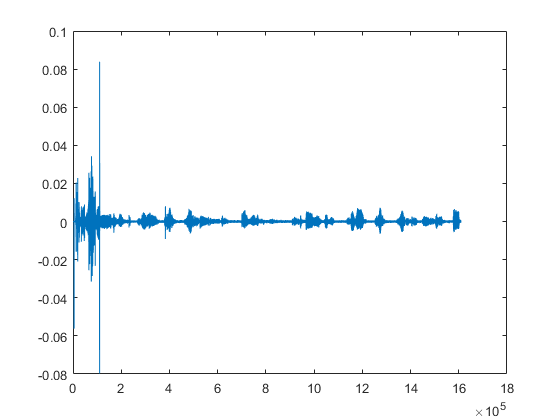
\includegraphics[scale=0.6]{Erreur.png}
\caption{Echo résiduel après filtrage.}
\label{echoAnnule}
\end{subfigure}
\begin{subfigure}{.5 \textwidth}
\centering
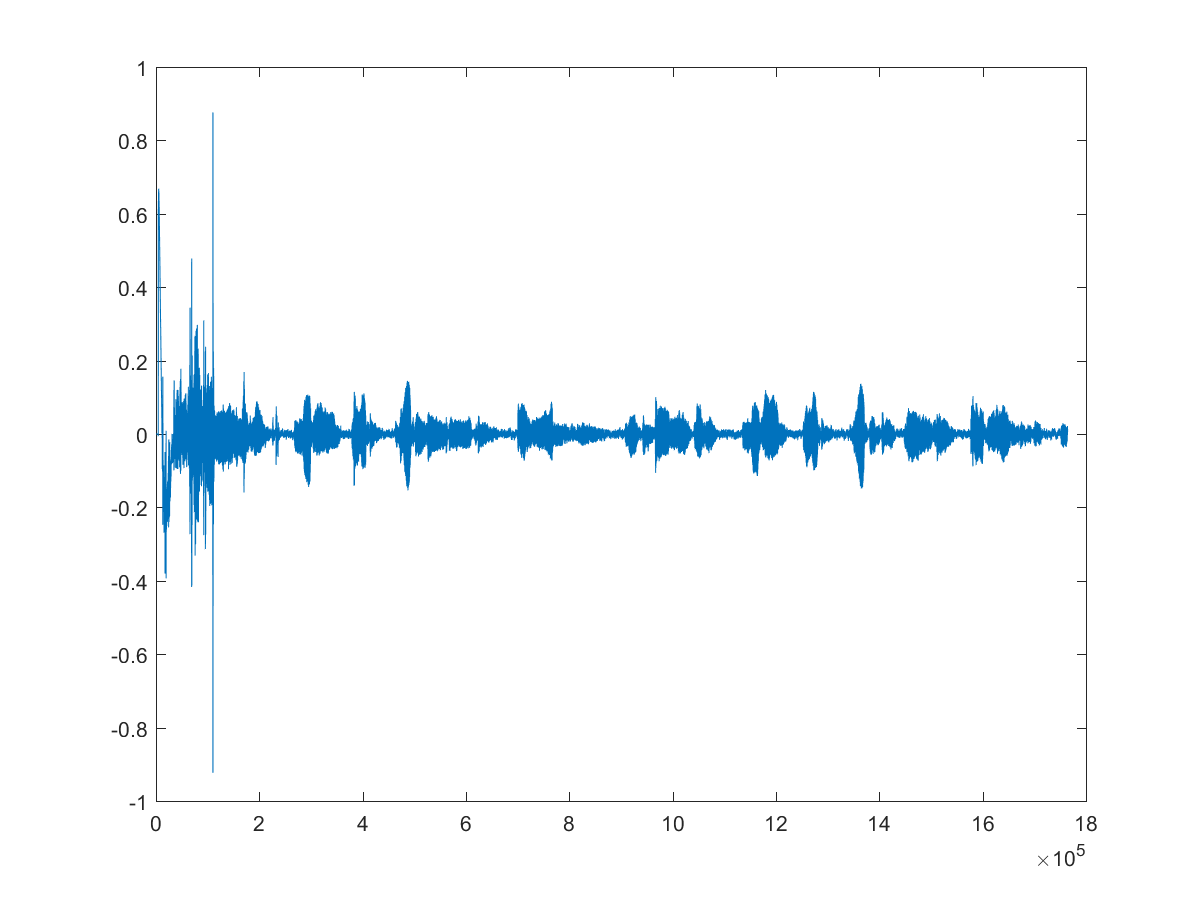
\includegraphics[scale=0.45]{Entree.png}
\caption{Echo sans filtrage.}
\label{echoNonAnnule}
\end{subfigure}
\caption{Démonstration de l'annulation d'écho}
\label{Annulation}
\end{figure}
Dans cette figure (la figure \ref{Annulation}), nous comparons l'écho reçu après filtrage du signal à envoyer à l'interlocuteur lointain, avec l'écho qu'il recevrait si le filtage n'était pas préalablement réalisé. Plus précisément, on réalise un filtrage pour modéliser l'écho, puis on le soustrait du signal à transmettre pour que l'interlocuteur lointain ne perçoive pas sa voix dans le signal qu'il recevra. Ainsi, en observant très bien les échelles des axes de ces figures, on remarque une atténuation très importante de l'écho. En effet, l'écho qui persiste après filtrage (voir la figure \ref{echoAnnule}) est environ le \emph{\textbf{dixième}} de celui qui est perçu lorsqu'aucun filtrage n'est réalisé \ref{echoNonAnnule}. Et on y voit très bien que pour ce dernier cas (absence de filtrage) l'interlocuteur lointain va entendre exactement son signal lui revenir. D'où la nécessité du filtrage.
\section{Conclusion partielle}
Dans cette dernière partie, nous avons tout d'abord décrit les éléments principaux nécessaires à l'élaboration d'un système annulateur d'écho sans prendre en compte le fait qu'il peut être incorporé à un système déjà mis en place. C'est ainsi que nous avons vu en passant la chaîne de traitement du signal et finalement nous nous sommes focalisé sur la partie concernant le traitement proprement-dit par filtrage. Cela nous a conduit à élaborer l'algorithme d'adaptation des coefficients du filtre de manière détaillée sous \textbf{Matlab} en vu d'en évaluer le fonctionnement et l'adéquation aux résultats attendus. Et bien évidemment, nous nous attendions à un filtre semblable à une impulsion  et nous l'avions obtenu de très près comme le prévoit la théorie. Nous avons finalement terminé par une illustration de l'annulation d'écho et une explication de l'implantation de l'algorithme sur DSP en système indépendant.
\chapter*{CONCLUSION GÉNÉRALE}\addcontentsline{toc}{chapter}{CONCLUSION GÉNÉRALE}
Au début de ce travail, nous pensions devoir considérer en profondeur les phénomènes physiques sous-jacents à la propagation des ondes sonores. Au cours des recherches, nous nous sommes rendu bien compte qu'il était plus rapide et rentable de modéliser juste l'ensemble, pour pouvoir mener à bien le travail à un coût dérisoire. Il est en effet plus optimal de traiter les phénomènes complexes, comme les phénomènes de propagation du son en dehors des conditions de laboratoire, de manière approximative mais globale au lieu de les voir en détail. Comme cela a bien été souligné, l'approche détaillée est utopique vu que le coût de calcul est immensément énorme.\\
En introduction, nous avons posé comme hypothèse, que le filtrage est une solution à la présence indésirée d'écho dans un système de communication, et ce travail vient évidemment de nous conforter dans cette affirmation. Nous avons également supposé qu'un filtrage purement analogique serait moins rentable mais nous nous sommes rendu compte au fil du travail que, cette proposition doit être bien nuancée. En effet, durant ce travail, nous avons montré que nous ne pouvons, si nous considérons le système dans son ensemble (et non seulement la partie qui concerne le traitement algorithmique), nous passer d'une partie de traitement analogique du signal (penser au filtre anti-repliement par exemple). Néanmoins, en nous basant uniquement sur le filtrage du signal reçu, sans trop nous fier au formatage et à la correction du rapport signal sur bruit, nous pouvons sans doute nous fier uniquement à un traitement purement numérique. Finalement, au vu du processus mis en œuvre pour l'adaptation du filtre annulateur d'écho, nous confirmons la troisième hypothèse lancée en introduction et affirmant qu'on ne peut se passer d'une mémorisation dynamique du signal durant une partie du traitement pour pouvoir mener à bien l'annulation de l'écho sonore lié au système de communication.
\paragraph{}
Ce travail a pointé du doigt la puissance de la théorie mathématique de traitement du signal. C'est ainsi  qu'il a pu déboucher sur le filtrage numérique et en premier lieu sur le filtrage de Wiener qui est évidemment un prélude inévitable pour aborder le filtrage adaptatif.\\
Le filtrage adaptatif car, comme cela a été plusieurs fois mentionné, c'est le moyen par excellence pour pouvoir modéliser un système non stationnaire comme c'est le cas pour les systèmes sonores. Notre travail a donc consisté à élaborer un filtre numérique modélisant l'enceinte dans laquelle le son va se propager, de telle sorte qu'il ne puisse pas y avoir une grande différence entre le son perçu à la sortie du filtre et celui qui serait perçu après avoir parcouru la salle. Cela revient donc à modéliser le chemin d'écho. Pour cela, les coefficients du filtre élaboré doivent correspondre à la réponse impulsionnelle de l'enceinte (à l'endroit où l'on se tient pour la mesurer).\\
Toutefois, les signaux sonores étant très instationnaires, il est impérieux d'adapter ces coefficients au fur et à mesure de la réception du signal. D'où la nécessité des filtres adaptatifs comme on l'a tantôt montré. Nous avons développé les algorithmes du filtrage adaptatif en nous focalisant sur les plus indiqués pour l'identification des système (le chemin d'écho pour notre cas). Cela nous a conduit à considérer un algorithme nommé \textbf{PNLMS++} qui est très indiqué dans des tels systèmes pour sa grande vitesse de convergence et sa robustesse.\\
L'objectif visé est qu'en cas de besoin, les théories abordées dans ce travail puissent être exploitées directement pour élaborer des systèmes devant équiper des appareils de communication habituels pour l'annulation d'échos sonores éventuels. C'est pour cette raison qu'il nous a semblé très important de montrer de quelle manière on pourrait réduire toujours plus fortement la charge de calcul des processeurs numériques à utiliser ainsi que le coût (d'un point de vu pécuniaire) de l'ensemble. De toute évidence, les processeurs à virgule fixe sont les plus adaptés à l'élaboration des plate-formes à faible prix tout en gardant une efficacité admissible quand ils sont programmés en conséquence. Ils allient en fait la rentabilité financière à la précision en ce qui concerne notre projet. Ce qui précède justifie le choix d'un traitement tout à fait particulier des données pour les rendre adaptées le plus fortement possible aux processeurs à virgule fixe (il s'agit du traitement par transformation en nombres de Fermat en lieu et place de la transformation de Fourier). Cette nouvelle transformation a toutes les propriétés nécessaires pour développer et optimiser la majorité des processus d'annulation d'écho dès qu'on décide de les implanter sur un processeur à virgule fixe.\\
Au préalable, nous prévoyions réaliser les algorithmes en langage C mais nous étant rendu compte du fait que cela serait sans intérêt( en première approximation), nous avons choisi de développer le système sous Matlab sachant que si on envisageait une implantation sur DSP, l'adaptation du code serait simple étant donné la similarité des syntaxes de ces deux langages. C'est sous cet angle que nous avons mis au point sous Matlab un algorithme complet d'adaptation des coefficient du filtre destiné à l'annulateur d'écho.\\
Aux futurs chercheurs, nous suggérons l'étude complète de l'incorporation des algorithmes ici conçus, aux systèmes de communication complets ainsi que, la correction des erreurs introduites dans le filtre obtenu en cas de traitement par blocs, pour améliorer encore plus l'atténuation de l'écho par cette méthode vu que ce dernier traitement est le mieux adapté au fonctionnement en temps réel.

\backmatter
%\appendix
\bibliographystyle{unsrt}
\bibliography{Bibliographie}
\backmatter
%\appendix
\begin{appendices}
\section{Algorithme de traitement brut}\label{Anne1}
\begin{verbatim}
1  -	%Récupération du son
2  -	
3  -	%Définition de la période d'échantillonnage
4  -	fs=44100;
5  -	%Définition du nombre de voies d'enregistrement
6  -	noc=1;
7  -	%Définition du nombre de bits
8  -	nob=16;
9  -	%Enregistrement du signal audio
10 -	recObj=audiorecorder(fs,nob,noc);
11 -	record(recObj);
12 -	pause(40);
13 -	stop(recObj);
14 -	%Lancement du signal enregistré
15 -	play(recObj);
16 -	%Formatage du signal enregistré sous forme vectoriel
17 -	myrecordings=getaudiodata(recObj);
18 -	%Représentation du signal enregistré
19 -	plot(myrecordings);
20 -	%Fin de la partie prise de son
21 -	
22 -	%Début de l'algorithme et lancement du chronométrage
23 -	tic;
24 -	%Initialisations et déclaration des constantes
25 -	
26 -	yk=ones(1,64);
27 -	%Déclaration des constantes "beta", "delta", "rho" et "mu".
28 -	b=100;
29 -	D=(1/64);
30 -	rho=0.01;
31 -	mu=0.8;
32 -	%Initialisation des W pour NLMS puis PNLMS.
33 -	w1=(ones(1,64))';
34 -	w2=(ones(1,64))';
35 -	%Initialisation des vecteurs utiles au calcul de Gk.
36 -	gam=zeros(1,64);
37 -	gk=zeros(1,64);
38 -	%Initialisation des vecteurs d'erreur et de W.
39 -	err=(1:64000);
40 -	w=zeros(1:64);
41 -	
42 -	%Début du traitement
43 -	for i=1:20850
44 -	    %Récupération du vecteur d'entrée à chaque étape i
45 -	    sign=(myrecordings((64+(i-1)):-1:(1+(i-1))))';
46 -	    
47 -	    %Calcul d'un paramètre utile pour trouver le vecteur Gk
48 -	    Vk=max([D,abs(w)]);
49 -	    %Calcul du vecteur Gk
50 -	    for k=1:64
51 -	        gam(k)=max(((rho)*Vk),(abs(w(k))));
52 -	    end
53 -	    for M=1:64
54 -	        gk(M)=((gam(M))/(mean(gam)));
55 -	    end
56 -	    Gk=1*diag(gk);
57 -	    %Calcul des éléments du vecteur d'erreur en gérant le début
58 -	    for s=1+(i-1):64+(i-1)
59 -	        sign2=(myrecordings((64+(s-1)):-1:(1+(s-1))))';
60 -	        yk(s) = (sign2)*w';
61 -	        err(s+63)=((yk(s)-myrecordings(64+(s-1))));
62 -	    end
63 -	    
64 -	    %Début du processus de réinitialisation du filtre
65 -	    
66 -	    %Algorithme PNLMS (Calcul du vecteur W1)
67 -	        w1=(w'+(mu*Gk*((sign)')*err(i+63))/(sign*Gk*(sign)'+b)));
68 -	    %Algorithme NLMS (Calcul du vecteur W2)    
69 -	        w2=(w'+((mu*((sign)')*err(i+63))/(((sign)*((sign)')+b))));
70 -	        
71 -	        
72 -	    %Réinitialisation des coefficients du filtre par PNLMS++
73 -	    
74 -	    for k=1:64
75 -	        %Coefficients impairs par PNLMS
76 -	        if mod(k,2)==1
77 -	          w(k)=w1(k);
78 -	        %Coefficients pairs par NLMS
79 -	        elseif mod(k,2)==0
80 -	            w(k)=w2(k);
81 -	        end
82 -	    end
83 -	end
84 -	%Fin du chronométrage
85 -	toc;
\end{verbatim}
\textbf{Revenir dans le texte en cliquant \ref{Brut}}.
\section{Algorithme de traitement par blocs}\label{Anne2}
\begin{verbatim}
1   -	%Récupération du son
2   -	
3   -	%Définition de la période d'échantillonnage en respectant Shannon
4   -	fs=44100;
5   -	%Définition du nombre de voies d'enregistrement
6   -	noc=1;
7   -	%Définition du nombre de bits
8   -	nob=16;
9   -	%Enregistrement du signal audio
10  -	recObj=audiorecorder(fs,nob,noc);
11  -	record(recObj);
12  -	pause(40);
13  -	stop(recObj);
14  -	%Lancement du signal enregistré
15  -	play(recObj);
16  -	%Formatage du signal enregistré sous forme vectoriel
17  -	myrecordings=getaudiodata(recObj);
18  -	%Représentation du signal enregistré
19  -	plot(myrecordings);
20  -	%Fin de la partie prise de son
21  -	
22  -	%Début de l'algorithme et lancement du chronométrage
23  -	tic;
24  -	%Initialisations et déclaration des constantes
25  -	
26  -	w=zeros(1,64);
27  -	zero=zeros(1,64);
28  -	%Complément de W par des zeros pour atteindre la longueur réquise
29  -	wk=[w,zero]';
30  -	%Déclaration des constantes "beta", "delta", "rho" et "mu".
31  -	b=100;
32  -	D=(1/64);
33  -	rho=(10^(-2));
34  -	mu=(0.8);
35  -	%Initialisation des W pour BNLMS puis BPNLMS.
36  -	w1=(ones(1,64))';
37  -	w2=(ones(1,64))';
38  -	%Initialisation des vecteurs utiles au calcul de Gk.
39  -	gam=zeros(1,64);
40  -	gk=zeros(1,64);
41  -	
42  -	%Début du traitement
43  -	for i=1:20850
44  -	    %Sélection particulier du premier bloc d'échantillons
45  -	    if i==1
46  -	        sign=(myrecordings(1:128))';
47  -	        sign2=(myrecordings(128:-1:1));
48  -	    %Sélection général de tous les blocs    
49  -	    elseif i>=2
50  -	        sign=(myrecordings(65+64*(i-2):192+64*(i-2)))';
51  -	        sign2=(myrecordings((192+64*(i-2)):-1:(65+64*(i-2))));
52  -	    end
53  -	    
54  -	    %Transformation du signal d'entrée et du vecteur W
55  -	    SIG=fft(sign);
56  -	    W=(fft(wk))';
57  -	    %Calcul du produit terme à terme des deux vecteurs
58  -	    Y=SIG.*W;
59  -	    %Transformation inverse pour retrouver le produit de convolution
60  -	    YW=ifft(Y);
61  -	    %Sélection des termes utiles recherchés
62  -	    yw=YW(65:128);
63  -	    %Calcul du vecteur d'erreurs
64  -	    err=(myrecordings(1+64*(i-1):64*i))'-(yw);
65  -	    %Complément du vecteur par des zeros puis transformation
66  -	    ERR=[err,zero];
67  -	    errF=fft(ERR);
68  -	    %Transformation du vecteur image
69  -	    SIG2=fft(sign2);
70  -	    %Réalisation de l'étape 3°) points 15, 16 et 17 de l'algorithme
71  -	    ERsign=(errF)'.*(SIG2);
72  -	    erSIGN=ifft(ERsign);
73  -	    es=erSIGN(65:128);
74  -	    %Réalisation de l'étape 3°) points 18 et 19 (autocorrélation)
75  -	    RSS=SIG2.*(SIG)';
76  -	    RSs=ifft(RSS);
77  -	    Rss=RSs(65:128);
78  -	    
79  -	    %Calcul d'un paramètre utile pour trouver le vecteur Gk
80  -	    Vk=max([D,abs(w)]);
81  -	    %Calcul du vecteur Gk
82  -	    for k=1:64
83  -	        gam(k)=max(((rho)*Vk),(abs(w(k))));
84  -	    end
85  -	    for M=1:64
86  -	        gk(M)=((gam(M))/(mean(gam)));
87  -	    end
88  -	    Gk=diag(gk);
89  -	    %Réalisation de l'étape 3°) point 21
90  -	    GkRss=Gk*(Rss);
91  -	    
92  -	    GkEsi2=Gk*es;
93  -	    
94  -	    %Réinitialisation des coefficients du filtre
95  -	    
96  -	    for j=1:64
97  -	        %Algorithme BPNLMS
98  -	        w1(j)=(w(j)+((mu*GkEsi2(j))/(GkRss(j)+b)));
99  -	        %Algorithme BNLMS
100 -	        w2(j)=(w(j)+((mu*es(j))/(Rss(j)+b)));
101 -	        
102 -	        %Réinitialisation des coefficients du filtre par BPNLMS++
103 -	        %Coefficients impairs par BPNLMS
104 -	        if mod(j,2)==1
105 -	            w(j)=w1(j);
106 -	        %Coefficients pairs par BNLMS    
107 -	        elseif mod(j,2)==0
108 -	            w(j)=w2(j);
109 -	        end
110 -	    end
111 -	end
112	-	w=((ones(1,64))*(13.5)-(w))/(13.5);
113 -	%Fin du chronométrage
114 -	toc;
\end{verbatim}
\textbf{Revenir dans le texte en cliquant \ref{Bloc}}.
\end{appendices}
\end{document}